\documentclass[fontsize=12pt,
% headinclude,
 twoside=false, parskip=half+, numbers=noenddot, plainheadsepline, toc=listof
 %, toc=bibliography
 ]{scrreprt}
% PDF-Kompression
\pdfminorversion=5
\pdfobjcompresslevel=1
% Allgemeines
\usepackage[automark]{scrpage2} % Kopf- und Fußzeilen
\usepackage{amsmath,marvosym} % Mathesachen
\usepackage[T1]{fontenc} % Ligaturen, richtige Umlaute im PDF
\usepackage[utf8]{inputenc}% UTF8-Kodierung für Umlaute usw

\usepackage{geometry}
\geometry{a4paper,left=50mm,right=30mm, top=1cm, bottom=2cm}
% Schriften
\usepackage{mathpazo} % Palatino für Mathemodus
%\usepackage{mathpazo,tgpagella} % auch sehr schöne Schriften
\usepackage{setspace} % Zeilenabstand
\onehalfspacing % 1,5 Zeilen
% Schriften-Größen
\setkomafont{chapter}{\Large\rmfamily} % Überschrift der Ebene
\setkomafont{section}{\large\rmfamily}
\setkomafont{subsection}{\rmfamily}
\setkomafont{subsubsection}{\rmfamily}
\setkomafont{chapterentry}{\large\rmfamily} % Überschrift der Ebene in Inhaltsverzeichnis
\setkomafont{descriptionlabel}{\bfseries\rmfamily} % für description Umgebungen
\setkomafont{captionlabel}{\small\bfseries}
\setkomafont{caption}{\small}
% Sprache: Deutsch
\usepackage[ngerman]{babel} % Silbentrennung
% PDF
\usepackage[ngerman]{hyperref}
\usepackage[final]{microtype} % mikrotypographische Optimierungen
\usepackage{url}
\usepackage{pdflscape} % einzelne Seiten drehen können
% Tabellen
\usepackage{multirow} % Tabellen-Zellen über mehrere Zeilen
\usepackage{multicol} % mehre Spalten auf eine Seite
\usepackage{tabularx} % Für Tabellen mit vorgegeben Größen
\usepackage{longtable} % Tabellen über mehrere Seiten
\usepackage{array}
%  Bibliographie
%\usepackage{bibgerm} % Umlaute in BibTeX
% Tabellen
\usepackage{float}
\usepackage{wrapfig}
% Bilder
\usepackage{graphicx} % Bilder
\usepackage{color} % Farben
\usepackage{colortbl}%Hintergrundfarben für Tabellen	
% Define user colors using the RGB model
\definecolor{dunkelgrau}{rgb}{0.8,0.8,0.8}
\definecolor{hellgrau}{rgb}{0.95,0.95,0.95}
\definecolor{red}{rgb}{1.0,0.5,0.5}
\graphicspath{{images/}}
\DeclareGraphicsExtensions{.pdf,.png,.jpg} % bevorzuge pdf-Dateien
\usepackage{subfigure} % mehrere Abbildungen nebeneinander/übereinander
\newcommand{\subfigureautorefname}{\figurename} % um \autoref auch für subfigures benutzen
\usepackage[all]{hypcap} % Beim Klicken auf Links zum Bild und nicht zu Caption gehen
% Bildunterschrift
\setcapindent{0em} % kein Einrücken der Caption von Figures und Tabellen
\setcapwidth[c]{0.9\textwidth}
\setlength{\abovecaptionskip}{0.2cm} % Abstand der zwischen Bild- und Bildunterschrift
% Quellcode
\usepackage{listings} % für Formatierung in Quelltexten
\definecolor{grau}{gray}{0.25}
\definecolor{lightgray}{rgb}{.9,.9,.9}
\definecolor{darkgray}{rgb}{.4,.4,.4}
\definecolor{purple}{rgb}{0.65, 0.12, 0.82}

\lstdefinelanguage{JavaScript}{
  keywords={typeof, new, true, false, catch, function, return, null, catch, switch, var, if, in, while, do, else, case, break},
  keywordstyle=\color{blue}\bfseries,
  ndkeywords={class, export, boolean, throw, implements, import, this},
  ndkeywordstyle=\color{darkgray}\bfseries,
  identifierstyle=\color{black},
  sensitive=false,
  comment=[l]{//},
  morecomment=[s]{/*}{*/},
  commentstyle=\color{purple}\ttfamily,
  stringstyle=\color{red}\ttfamily,
  morestring=[b]',
  morestring=[b]"
}
\lstset{
   language=JavaScript,
   backgroundcolor=\color{lightgray},
   extendedchars=true,
   basicstyle=\scriptsize\ttfamily,
   showstringspaces=false,
   showspaces=false,
   %numbers=right,
   numberstyle=\scriptsize\ttfamily,
   numbersep=9pt,
   tabsize=2,
   breaklines=true,
   showtabs=false,
   captionpos=b
}
%\lstset{
%	extendedchars=true,
%	%basicstyle=\small\ttfamily,
%	language=java,
%	basicstyle=\footnotesize\ttfamily,
%	tabsize=2,
%	keywordstyle=\textbf,
%	commentstyle=\color{grau},
%	stringstyle=\textit,
%	numbers=left,
%	numberstyle=\small,
%	% für schönen Zeilenumbruch
%	breakautoindent  = true,
%	breakindent      = 2em,
%	breaklines       = true,
%	postbreak        = ,
%	prebreak         = \raisebox{-.8ex}[0ex][0ex]{\Righttorque},
%}
% linksbündige Fußboten
\deffootnote{1.5em}{1em}{\makebox[1.5em][l]{\thefootnotemark}}

%\typearea{14} % typearea am Schluss berechnen lassen, damit die Einstellungen oben berücksichtigt werden
% für autoref von Gleichungen in itemize-Umgebungen
\makeatletter
\newcommand{\saved@equation}{}
\let\saved@equation\equation
\def\equation{\@hyper@itemfalse\saved@equation}
\makeatother 


 % Importiere die Einstellungen aus der Präambel
% hier beginnt der eigentliche Inhalt
\begin{document}
\pagenumbering{Roman} % große Römische Seitenummerierung
\pagestyle{empty}

% Titelseite
\clearscrheadings\clearscrplain

\begin{center}
\begin{Huge}
Institut für Mathematik und Informatik\\
\vspace{3mm}
\end{Huge}{\Large Fernuniversiät Hagen}\\

\vspace{20mm}
\begin{Large}
Vergleichende Implementierung und Evaluierung einer ereignisgesteuerten, nicht
blockierenden I/O Lösung für eine datenintensive Real-Time Webanwendung in Javascript
und Dart\\
\end{Large}
\vspace{8mm}
Bachelorarbeit\\
\vspace{0.4cm}
\vspace{2 cm}
Barbara Drüke \\
Matrikel-Nummer 7397860\\
\vspace{5cm}
\begin{tabular}{ll}
{\bf Betreuer} & Dr. Jörg Brunsmann\\
{\bf Erstprüfer}&Prof. Hemmje\\
{\bf Zweitprüfer}&Dr. Jörg Brunsmann\\
\end{tabular}

\end{center}
\clearpage


\pagestyle{useheadings} % normale Kopf- und Fußzeilen für den Rest

\tableofcontents
\listoffigures
\listoftables
\lstlistoflistings





% richtiger Inhalt
%---------------------------------------------------------------------------------------------------------------------------------------------
\chapter{Einleitung}
\pagenumbering{arabic} % ab jetzt die normale arabische Nummerierung

Die Vesseltracker.com GmbH ist ein Schiffsmonitoring und -reporting-Dienstleister. Der kostenpflichtige Dienst stellt den Kunden umfangreiche Informationen zu Schiffen weltweit zur Verfügung. Dabei handelt es sich einerseits um Schiffs-Stammdaten und andererseits um Schiffs-Postionsdaten. Die Positionsdaten sind AIS (Automatic Identification System) -Daten, wie sie von allen Schiffen über Funk regelmäßig zu senden sind.

\begin{wrapfigure}{r}{0.6\textwidth}
  \begin{center}
    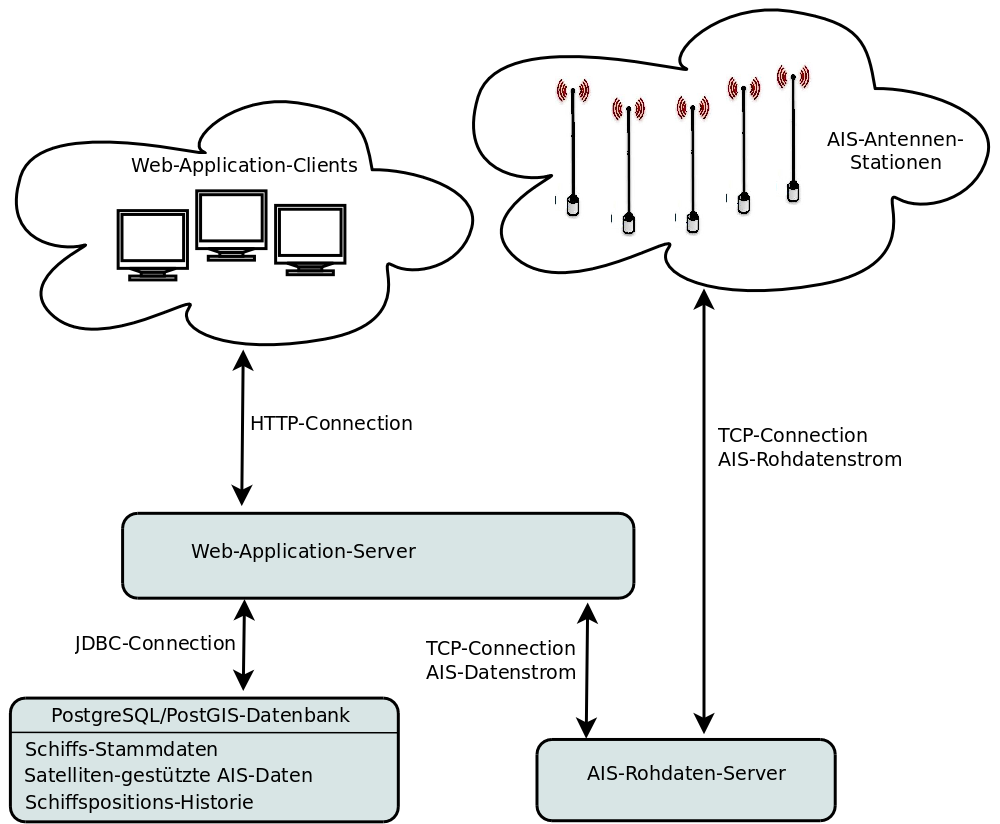
\includegraphics[width=0.58\textwidth]{images/Exposee_graphik_Webapp}
  \end{center}
  \caption{Architektur der Web-Anwendung der Vesseltracker.com-GmbH}
\end{wrapfigure}

Vesseltracker.com unterhält ein Netzwerk von ca. 800 terrestrischen AIS-Antennen, mit denen küstennahe AIS-Meldungen empfangen und via Internet an einen zentralen Rohdatenserver geschickt werden. Der Rohdatenserver verarbeitet die Meldungen und gibt sie umgewandelt und gefiltert an die Anwendungen des Unternehmens weiter.
Zusätzlich erhält das Unternehmen AIS-Daten via Satellit über einen Kooperationspartner. Damit werden die küstenfernen Meeresgebiete und Gegenden, in denen Vesseltracker.com keine AIS-Antenne betreibt, abgedeckt.
Die Kernanwendung des Unternehmens ist eine Webanwendung, die die terrestrischen AIS-Daten in einer Geo-Datenbank speichert und sie mit den Schiffs-Stammdaten und Satelliten-AIS-Daten in Beziehung setzt.

Für eine geographische Visualisierung der Schiffspositionen existiert das sogenannte 'Cockpit', wo die Schiffe als Icons auf Openstreetmap-Karten dargestellt werden. Diese Karte zeigt jeweils alle Schiffe an, die sich in dem frei wählbaren Kartenausschnitt zu der Zeit befinden. Aktualisiert werden die Positionsinformationen jeweils bei Änderung des betrachteten Bereichs oder einmal pro Minute. Detailinformationen erhält der Nutzer durch ein Click-Popup über das Icon des Schiffes. Darüber kann er sich auch die gefahrene Route der letzten 24 Stunden anzeigen lassen.


\begin{figure}[H]
  \centering
  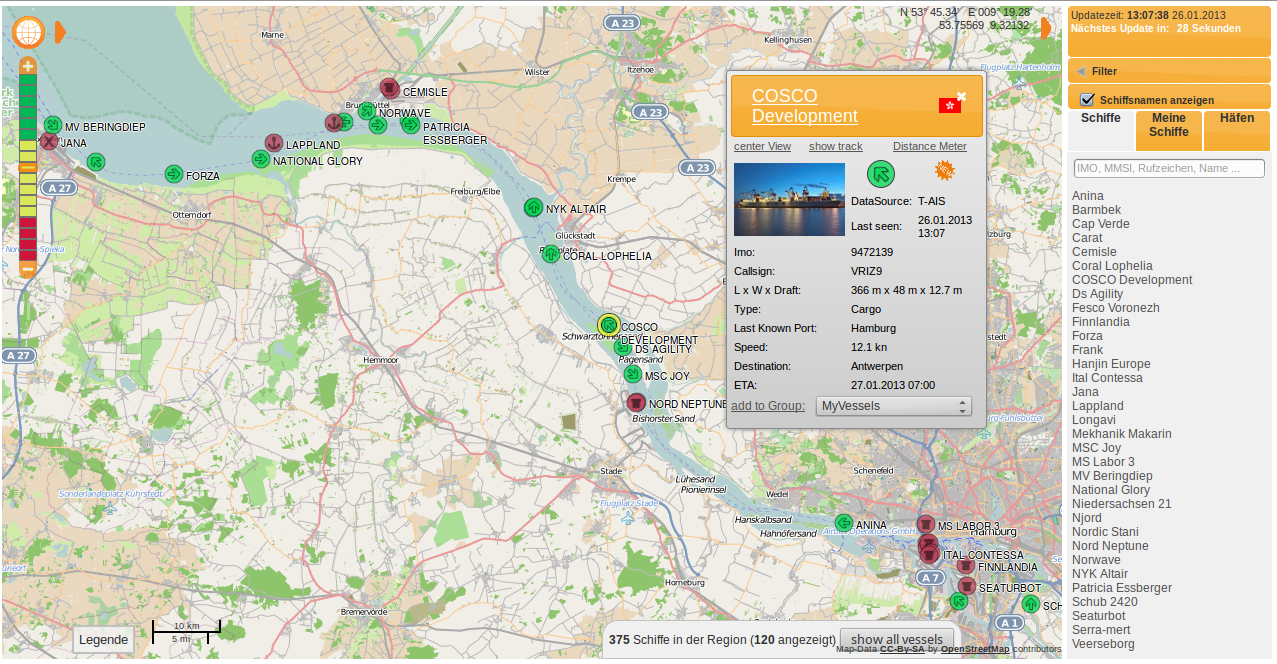
\includegraphics[width=6in]{images/Cockpit_Elbe}
  \caption[Ansicht der Elbe hinter Hamburg in der ‘Cockpit’-Anwendung]{Ansicht der Elbe hinter Hamburg in der ‘Cockpit’-Anwendung}
\end{figure}

\section{Motivation für diese Arbeit}\label{s.Motivation für diese Arbeit}

Aus mehreren Gründen entstand der Plan, dem Portfolio des Unternehmens neben der existierenden Cockpit-Anwendung eine Real-Time-Darstellung der geographischen Schiffspositionen hinzuzufügen.
\begin{itemize}

\item Aufgrund der herausragenden Qualität des vesseltracker.com Antennen-Netzwerks sind die verfügbaren terrestrischen AIS-Daten höchst aktuell, aktualisieren sich kontinuierlich und erreichen eine hohe weltweite Abdeckung des Schiffsverkehrs. Damit ist es möglich, die Situation des Schiffsverkehrs in beliebigen Häfen, Wasserstraßen und Küstengebiete weltweit und sekundengenau zu präsentieren. Diese Genauigkeit wird in der Cockpit-Anwendung nicht vollständig genutzt.

\item Real-Time-Anwendungen gewinnen laufend an Bedeutung. Ihre Verbreitung wird durch den Fortschritt der verfügbaren Webtechnologien auf breiter Basis unterstützt. Mitbewerber auf dem Markt für AIS-Daten (z.B. Fleetmon.com) bieten bereits Echtzeit-Darstellungen ihrer AIS-Daten an. Um in diesem Geschäftsfeld weiterhin eine Spitzenposition beanspruchen zu können, sollte auch Vesseltracker eine Real-Time-Anwendung zur Schiffsverfolgung für Desktop-Computer zur Verfügung stellen und in einem nächsten Schritt auch für Mobile Devices.
\item Ein Phänomen in der menschlichen Wahrnehmung liefert ein weiteres Argument, die Cockpit-Anwendung durch eine Real-Time-Anwendung zu ergänzen oder sogar abzulösen: Aufgrund der sogenannten Veränderungsblindheit oder “Change Blindness” werden Veränderungen an einem Objekt (in diesem Fall die Position eines Schiffs-Icons auf der Karte) in der Wahrnehmung überdeckt, wenn im selben Augenblick Veränderungen an der Gesamtsicht vonstatten gehen \cite{changeblindness}. Genau dies geschieht im Cockpit, wenn nach dem Laden neuer Positionsdaten alle Schiffs-Icons neu gerendert und Namens-Fähnchen gelöscht oder hinzugefügt werden. Dieses kurze “Flackern” macht es dem Betrachter fast unmöglich, die Positionsänderung eines Schiffes auf der Karte mit dem Auge zu verfolgen.
\end{itemize}


\section{Aufbau der Arbeit}\label{s.Aufbau der Arbeit}
Im Kapitel \ref{c.Realtime-Schiffsverfolgung per AIS-Daten-Strom} werden mögliche Anwendungs-Szenarien genauer beleuchtet und die funktionalen und nicht funktionalen Anforderungen an die geplante Anwendung herausgestellt. Anschließend wird die Systemarchitektur der geplanten Anwendung grob entworfen.
In Kapitel \ref{s.Grundlagen} wird kurz auf die technischen Grundlagen eingegangen: die AIS-Technologie, die bei der Gewinnung des Datenmaterials verwendet wird und damit für Art und Format der Daten verantwortlich ist; das Javascript-Framework node.js sowie Google Dart, die bei der Programmierung der Anwendung zum Einsatz kommen; HTML5-Websockets, weil sie für die Verteilung der Daten eingesetzt werden; das OpenStreetMap-Projekt als Lieferant des Kartenmaterials wird kurz vorgestellt, sowie die Leaflet-Bibliotheken, mit deren Hilfe die Schiffsobjekte auf die Karte gerendert werden.

In Kapitel \ref{s.Implementierungen} werden zunächst die Gründe für die spezifische Auswahl an Implementierungen dargelegt. Anschließend wird die Vorgehensweise bei der Implementierung erläutert und zwar zunächst ausführlich für die jeweils erste Server- bzw. Client-Implementierung (socket.io-Server \ref{socket.io-Server} und socket.io-Client \ref{socket.io-Client}). Anschließend werden für die alternativen Implementierungen nur jeweils die Unterschiede herausgestellt. Die fertigen Programme werden in Kapitel \ref{Ergebnisse} getestet und nach verschiedenen Aspekten verglichen.
Kapitel \ref{Fazit} fasst die Ergebnisse zusammen und gibt einen Ausblick auf mögliche Weiterentwicklungen.

%---------------------------------------------------------------------------------------------------------------------------------------------

\chapter{Real-Time-Schiffsverfolgung per AIS-Daten-Strom}\label{c.Realtime-Schiffsverfolgung per AIS-Daten-Strom}

\section{ Anwendungsfälle}\label{s.Anwendungsfälle}

Hafendienstleister wie Schlepper, Lotsen oder Festmacher verschaffen sich über einen Monitor einen Überblick über die Arbeitsvorgänge in ihrem jeweiligen Heimathafen, z.B. welche Schlepper schleppen welches Schiff, wo gehen Lotsen an oder von Bord, welche Tanker betanken welche Schiffe, usw. Sie kontrollieren die Ausführung der eigenen Aufträge oder auch die der Mitbewerber.
Die Anwendung läuft hierbei eigenständig, das heißt, Zoomstufe und Kartenausschnitt ändern sich nicht oder nur selten. Es ist also notwendig, dass die Anwendung unabhängig von Benutzer-Interaktionen immer die aktuellsten verfügbaren Daten anzeigt.\\
Ein verwandter Anwendungsfall betrifft Nutzer, für die die Beobachtung, bzw. Überwachung bestimmter Wasserverkehrswege oder Häfen von besonderem Interesse ist. Dies trifft auf Sicherheitsorgane (z.B. die Wasserschutzpolizei), Schiffsfotografen und Nutzer der Passagierschifffahrt zu.\\
Reedereien beobachten das Einlaufen, Anlegen, Festmachen oder Ablegen und Auslaufen ihrer Schiffe in entfernten Häfen, wo es keine Unternehmensniederlassung gibt. Zum Beispiel kontrollieren sie, wann und an welchen Liegeplätzen ein Schiff wie lange festmacht.
Dazu ist es zum einen notwendig, auf eine geringe Zoomstufe heraus- und auf einen anderen Hafen wieder hineinzoomen zu können. Zum anderen soll die Anwendung Schnittstellen bieten, um zusätzliche Informationen aus dem vesseltracker.com Datenpool (z.B. Liegeplatzinformationen) anzufordern.\\
Die vesseltracker.com GmbH nutzt die Real-Time-Anwendung, um die vom Unternehmen angebotenen Daten zu präsentieren und zu bewerben. Dabei ist es wichtig, dass die Anwendung gesendete AIS-Signale im Schnitt in weniger als einer Sekunde auf dem Monitor als Position oder Positionsänderung darstellen kann und dass die Schiffsbewegungen fließend ohne  “Flackern” dargestellt werden. Damit kann vesseltracker.com die größere Genauigkeit und Aktualität der eigenen Daten gegenüber denen anderer Anbieter herausstellen.

Die Anwendungsfälle verdeutlichen noch einmal, dass der zusätzliche Nutzen der Real-Time-Anwendung gegenüber der Cockpit-Anwendung nicht ausschließlich in der höheren Aktualität liegt, denn die Daten im Cockpit sind ja ebenfalls im Minutenbereich aktuell. Ein wichtiger Vorteil liegt vielmehr in der Lebendigkeit der Darstellung. Bewegte Objekte binden stärker die Aufmerksamkeit des Betrachters. Sie sind ohne Anstrengung mit dem Auge zu verfolgen und geben der Anwendung einen gewissen Unterhaltungswert.
\newpage
\section{Beschreibung der Anforderungen}\label{s.Beschreibung der Anforderungen}


\subsection{Funktionale Anforderungen}\label{Funktionale Anforderungen}
\begin{itemize}

\item als Datenquelle sollen ausschließlich die vom Rohdatenserver als JSON-Datenstrom zur Verfügung gestellten AIS-Informationen dienen
\item Schiffe sollen an ihrer aktuellen (Real-Time-) Position auf einer Karte im Browser dargestellt werden
\item Positionsänderungen einzelner Schiffe sollen ad hoc sichtbar gemacht werden
\item die Schiffsbewegungen auf der Karten sollen nicht sprunghaft, sondern fließend erscheinen (Animation der Schiffsbewegungen in dem Zeitraum zwischen zwei Positionsmeldungen)
\item die Karte soll in 16 Zoomstufen die Maßstäbe von 1:2000 bis 1: 200 Mio abdecken
\item Schiffe sollen auf der Karte als Symbole dargestellt werden, die den Navigationsstatus und gegebenenfalls den Kurs wiederspiegeln
\item bei hoher Auflösung / großem Zoom-Level und ausreichend statischen AIS-Informationen soll ein Schiff als maßstabsgetreues Polygon (genauer: Fünfeck) in die Karte gezeichnet werden.
\item bei geringer Auflösung / niedrigem Zoom-Level soll ein Eindruck über die Verteilung der empfangenen Schiffe vermittelt werden, ohne jedoch jedes Schiff tatsächlich darzustellen
\item Detail-Informationen zu jedem Schiff sollen als Popups über das Symbol auf der Karte abrufbar sein
\end{itemize}

\subsection{Nicht funktionale Anforderungen}\label{Nicht funktionale Anforderungen}
\begin{itemize}
\item die von den Antennen empfangenen AIS-Daten sind mit minimaler Verzögerung (unter 500 msec) auf der Karte darzustellen
\item die Anwendung soll ca. 300 gleichzeitige Client-Verbindungen erlauben und skalierbar sein
\item als Clients der Anwendung sollen die gängigen Browser in den am meisten verbreiteten Versionen unterstützt werden (Microsoft Internet Explorer, Google Chrome, Moziila Firefox, Apple Safari) 
\item der Programm-Code wird auf Github als privates repository gehostet
\item verwendete Software-Module sollen frei zugänglich (open source) sein 
\item als Kartenmaterial sind die von vesseltracker gehosteten OpenstreetMap-Karten zu verwenden
\item ein Prototyp der Anwendung soll zeitnah zur Verfügung stehen, um Mitarbeitern und Kunden zu ermöglichen, ihre Anforderungen genauer zu spezifizieren oder weitere Anforderungen zu formulieren.
\end{itemize}

\section{Grobentwurf der Anwendung}\label{s.Grobentwurf der Anwendung}

\begin{wrapfigure}{r}{0.6\textwidth}
  \begin{center}
    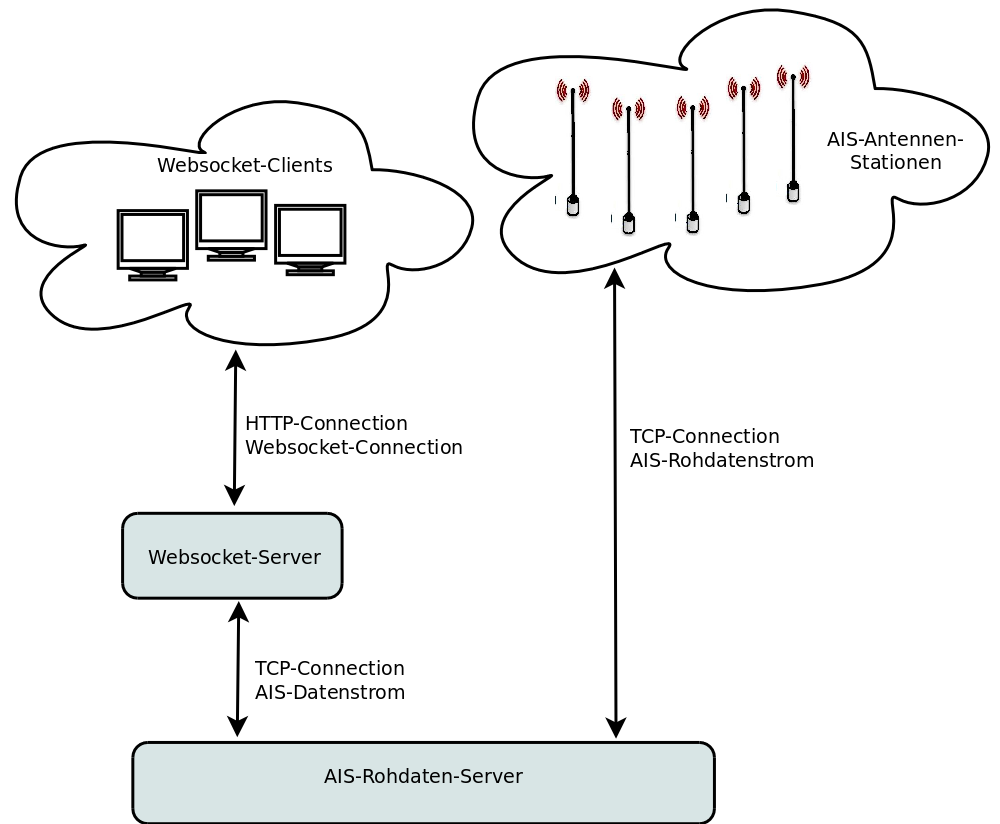
\includegraphics[width=0.6\textwidth]{images/Exposee_graphik_Realtimeapp}
  \end{center}
  \caption{Architektur-Entwurf der Real-Time Web-Anwendung}
\end{wrapfigure}
Die eingehende Schnittstelle der zu erstellenden Anwendung ist die Verbindung zum Rohdatenserver, die als TCP-Verbindung ausgeführt ist und einen JSON-Datenstrom liefert.
Die ausgehende Schnittstelle ist der HTTP-Client (Browser).
Zu erstellen ist also eine Client-Server-Anwendung, in der der Server zweierlei zu leisten hat, nämlich 
\begin{enumerate}
 \item eine TCP-Socket-Verbindung zum Rohdatenserver zur Abfrage des AIS-Daten-Stroms zu unterhalten und
  \item eine bidirektionale Verbindungen zu vielen HTTP-Clients herzustellen, in der die Clients Änderungen des betrachteten Kartenausschnittes an den Server senden können und der Server jederzeit den Client über relevante, aus dem JSON-Datenstrom ausgelesene, Schiffsbewegungen im betrachteten Kartenausschnitt informieren kann.
\end{enumerate}


%---------------------------------------------------------------------------------------------------------------------------------------------
\chapter{Grundlagen}\label{s.Grundlagen}
\section{Automatisches Informationssystem}\label{s.Automatisches Informationssystem (AIS)}
Das Automatic Identification System (AIS) ist ein UKW-Funksystem im Schiffsverkehr, das seit 2004 für alle Berufsschiffe über 300 BRZ ? in internationaler Fahrt und seit 2008 auch für solche über 500 BRZ in nationaler Fahrt verpflichtend eingeführt worden ist. Es soll dabei helfen, Kollisionen zwischen Schiffen zu verhüten und die landseitige Überwachung und Lenkung des Schiffsverkehrs zu erleichtern. Außerdem verbessert AIS die Planung an Bord, weil nicht nur Position, Kurs und Geschwindigkeit der umgebenden Schiffe übertragen werden, sondern auch Schiffsdaten (Schiffsname, MMSI-Nummer, Funkrufzeichen, etc.). AIS ist mit UKW-Signalen unabhängig von optischer Sicht und Radarwellenausbreitung \cite{wiki:ais}.\\
Für die Nutzung von AIS ist ein aktives, technisch funktionsfähiges Gerät an Bord Voraussetzung, das sowohl Daten empfängt als auch Daten sendet. Für Schiffe der Berufsschifffahrt sind Klasse-A-Transceiver an Bord vorgesehen, für nicht ausrüstungspflichtige Schiffe genügen Klasse-B-Transceiver, die mit niedriger VHF-Signalstärke und weniger häufig senden.  \\
Die dynamischen Schiffsdaten (s.u.) erhält der AIS-Transceiver vom integrierten GPS-Empfänger, bei Klasse A auch von der Navigationsanlage des Schiffes. Die Vorausrichtung (Heading) kann über eine NMEA-183-Schnittstelle vom Kompass eingespeist werden.

Die AIS-Einheit sendet schiffsspezifische Daten, die von jedem AIS-Empfangsgerät in Reichweite empfangen und ausgewertet werden können:
\subsubsection{Statische Schiffsdaten} \label{Statische Schiffsdaten}
\begin{itemize}
\item IMO-Nummer\footnote{http://de.wikipedia.org/wiki/Schiffsnummer\#IMO-Nummer}
\item Schiffsname
\item Rufzeichen\footnote{http://de.wikipedia.org/wiki/Schiffsnummer\#Unterscheidungssignal}
\item MMSI-Nummer\footnote{http://de.wikipedia.org/wiki/Schiffsnummer\#MMSI}
\item Schiffstyp (Frachter, Tanker, Schlepper, Passagierschiff, SAR, Sportboot u. a.)
\item Abmessungen des Schiffes (Abstand der GPS-Antenne von Bug, Heck, Backbord- und Steuerbordseite)
\end{itemize}

\subsubsection{Dynamische Schiffsdaten} \label{Dynamische Schiffsdaten}
\begin{itemize}
\item Navigationsstatus (unter Maschine, unter Segeln, vor Anker, festgemacht, manövrierunfähig u. a.)
\item Schiffsposition (LAT, LON in WGS 84)
\item Zeit der Schiffsposition (nur Sekunden)
\item Kurs über Grund (COG)
\item Geschwindigkeit über Grund (SOG)
\item Vorausrichtung (HDG)
\item Kursänderungsrate (ROT)
\end{itemize}

\subsubsection{Reisedaten} \label{Reisedaten}
\begin{itemize}
\item aktueller maximaler statischer Tiefgang in dm
\item Gefahrgutklasse der Ladung (IMO)
\item Reiseziel (UN/LOCODE)\footnote{http://www.unece.org/cefact/locode/service/location.html}
\item geschätzte Ankunftszeit (estimated Time of Arrival = ETA)
\item Personen an Bord
\end{itemize}

Der Navigationsstatus und die Reisedaten müssen vom Wachoffizier manuell aktualisiert werden. Gesendet werden die AIS-Signale auf zwei UKW-Seefunkkanälen (Frequenzen 161,975 MHz und 162,025 MHz), wobei die Sendeintervalle abhängig sind von der Klasse, dem Manöverstatus und der Geschwindigkeit.

\begin{table}[!hbt]\vspace{1ex}\centering
\small
\texttt{
\begin{tabular}{|l|l|l|l|}\hline
Klasse &Manöver-Status & Geschwindigkeit &Sendeintervall\\\hline\hline
Class A&geankert/festgemacht&<3kn&3 min\\
Class A&geankert/festgemacht&>3kn&10 sec\\
Class A&in Fahrt&0-14kn&10 sec\\
Class A&in Fahrt, Kursänderung&0-14&3 1/3 sec\\
Class A&in Fahrt&14-23kn&6 sec\\
Class A&in Fahrt, Kursänderung&14-23&2 sec\\
Class A&in Fahrt&>23kn&2 sec\\
Class B&&<2 kn&3 min\\
Class B&&>2 kn&30 sec\\\hline
\end{tabular}
}
\caption[Intervalle, in denen Schiffe AIS-Nachrichten aussenden] {Intervalle, in denen Schiffe AIS-Nachrichten aussenden}
\end{table}

Für AIS-Daten sind 22 standardisierte Nachrichtentypen bzw. Telegramme festgelegt. Für diese Arbeit interessieren nur die regulären Positionsmeldungen (dynamische Schiffsdaten) der Klasse-A-Transceiver (Typ 1- ,2-  und 3-Messages) und die regulären Meldungen von (statischen) Schiffs- und Reisedaten der Klasse-A-Transceiver (Typ 5-Messages). 
\section{OpenStreetMap}\label{OpenStreetMap}
OpenStreetMap\footnote{http://www.openstreetmap.org/} ist eine freie, editierbare Karte der gesamten Welt auf der Basis von Daten, die von einer breiten Nutzergemeinde zusammengetragen werden. Inzwischen kann die Qualität der Karten mit denen proprietärer Angebote mithalten und übertrifft sie sogar in manchen Bereichen. Die Daten können gemäß der entsprechenden Freien Lizenz frei heruntergeladen und genutzt werden unter der Bedingung, dass sie nur unter der “Creative Commons Attribution-Share-Alike” (CC-BY-SA) -Lizenz weitergegeben werden.

\section{Leaflet}\label{Leaflet}
Leaflet ist eine open source JavaScript-Bibliothek\footnote{http://leafletjs.com/reference.html} für interaktive Karten, die von einer Gruppe um Vladimir Agafonkin geschrieben wurde. Die Bibliothek zeichnet sich im Vergleich zu OpenLayers durch ein klares, schlankes Design aus und überzeugt durch gute Performance. Leaflet unterstützt alle Plattformen auch im mobilen Bereich mithilfe von HTML5 und CSS3. Es ist hinreichend dokumentiert und verfügt über gut lesbaren Quellcode.

\section{Bidirektionale Kommunikation über HTML5 Websockets}\label{s.Websockets}
In der Entwicklung der Kommunikationstechnologien im Internet galt lange Zeit das request/response Paradigma, nach dem Anfragen eines Clients von einem Server beantwortet werden. Dieses Paradigma wird Stück für Stück aufgebrochen durch kontinuierliche Weiterentwicklungen in Richtung einer bidirektionalen Kommunikation zwischen Server und Client.\\
Schon seit HTTP Long Polling, HTTP Streaming und Ajax on demand ist es für Serveranwendungen möglich, nach einem initialen Verbindungsaufbau durch den Client, beim serverseitigen Eintreffen neuer Daten scheinbar selbständig einen Datenaustausch zum Client zu initieren. Dabei handelt es sich eigentlich nur um die aufgeschobene Beantwortung einer zuvor gestellten Client-Anfrage.\\
Der Nachteil dieser Technologien liegt darin, dass sie, weil sie Nachrichten über das HTTP-Protokoll austauschen, einen großen Überhang an Header-Informationen mitzusenden gezwungen sind, der sich in Summe negativ auf die Latenzzeit auswirkt \cite{varaksin}. Damit sind diese Technologien für zeitkritische (Real-Time-) Anwendungen nicht unbedingt geeignet.
\\
Das 2011 eingeführte Websocket-Protokoll dagegen spezifiziert eine API (HTML5-Websocket API-Spezifikation \footnote{http://www.w3.org/TR/2011/WD-websockets-20110419/}), die eine echte bidirektionale Socket-Verbindung zwischen Server und Client ermöglicht, in der beide Seiten jederzeit Daten schicken können. Dieser Socket wird im Anschluss an einen intialen HTTP-handshake aufgebaut, indem Server und Client  einen Upgrade der Verbindung auf das Websocket-Protokoll aushandeln  \cite{html5rocks}. 

\section{node.js}\label{node.js}
Node.js\footnote{http://www.nodejs.org/} ist ein Framework zur Entwicklung serverseitiger Webanwendungen in Javascript. Es wurde 2009 von Ryald Dahl veröffentlich und hat seitdem viel Aufmerksamkeit erregt, weil Anwendungen in node.js
\begin{itemize}

\item hoch performant
\item skalierbar
\item und echtzeitfähig sind.
\end{itemize}

Diese Eigenschaften sind größtenteils dem Konzept des asynchronen, nicht blockierenden I/O von javascript im Allgemeinen und node.js im Besonderen geschuldet.
Javascript ist von Anfang asynchron konzipiert für die Verwendung im Webbrowser, wo synchrone Verarbeitung wegen der Verzögerung des Seitendarstellung nicht in Frage kommt. Den gleichen Ansatz übernimmt node.js für die Serverseite.
\\
Node.js arbeitet single-threaded und eventbasiert. Die zentrale Kontrollstruktur, die den Programmablauf steuert, ist der Event-Loop. Er empfängt Events, die von Programm- oder Nutzeraktionen ausgelöst werden und setzt sie in Callback-Funktionen um.
Kommt es im Programmablauf zur Interaktion mit einer externen Ressource, wird diese Interaktion in einen neuen Prozess ausgelagert und mit einer Callback-Methode versehen. Anschließend kann der Event Loop weitere aufgelaufene Events verarbeiten. Ist die Interaktion abgeschlossen bekommt der Event Loop ein Signal und setzt beizeiten die Verabeitung mit der entsprechenden Callback-Methode  fort \cite{teixeira}.\\
Node.js bringt als Laufzeitumgebung die V8-Javascript-Engine mit, die die Ausführung von Javascript-Code durch Just-In-Time-Kompilierung optimiert. Außerdem bietet node.js eine direkte Unterstützung für das HTML5-Websocket-Protokoll. Mit der Unterstützung des JSON-Datenformats sind alle notwendigen Bausteine zusammen für skalierbare, echtzeitfähige Serveranwendungen.
Außerdem lassen sich mit dem node.js Package Manager npm jederzeit weitere Pakete aus dem wachsenden Angebot nachinstallieren und verwalten.\\
Als konkrete Pakete für Websockets standen innerhalb von node.js zum Zeitpunkt der Implementierung (November 2012) die Bibliotheken websocket\footnote{https://github.com/Worlize/WebSocket-Node} und socket.io\footnote{http://socket.io} zur Verfügung. Die Bibliothek websocket genügt der HTML5-Websocket-Api-Spezifikation (s.o). Socket.io erweitert die Funktionalität des websockets um heartbeats, timeouts and disconnection support. Außerdem kapselt socket.io die Details des Nachrichtenaustauschs: Bei Browsern, die Websockets nicht unterstützen, handelt socket.io die bestmögliche Verbindungsalternative aus in der Reihenfolge: 
-->    WebSocket 
 -->   Adobe® Flash® Socket
  -->  AJAX long polling
   --> AJAX multipart streaming
 -->   Forever Iframe
 -->   JSONP Polling\footnote{http://socket.io/\#browser-support}.
Um socket.io zu nutzen können, muss im Browser-Client die Datei socket.io.js geladen werden.
\section{Google Dart}\label{s.Google Dart }

\subsubsection{Motivation für Dart}
Dart ist eine von der Firma Google als open source Projekt seit ca. 2 Jahren explizit für Webanwendungen entwickelte Programmiersprache. Das Ziel ist es, eine Sprache zu entwickeln, die komplexe Webanwendungen besser unterstützt als Javascript mit seinen historisch bedingten Mängeln und Schwächen.
Das Entwicklerteam definiert die Design-Ziele folgendermaßen\footnote{http://www.dartlang.org/docs/technical-overview/\#goals}:
Dart soll
\begin{itemize}   
\item eine sowohl strukturierte als auch flexible Web-Programmiersprache sein
\item sich für Programmierer vertraut anfühlen und intuitiv erlernbar sein 
\item mit seinen Sprachkonstrukten performant sein und schnell zur Ausführung kommen
\item auf allen Webdevices wie Mobiles, Tablets, Laptops und Servern gleichermaßen lauffähig sein
\item alle gängigen Browser unterstützen.
\end{itemize}

\subsubsection{Spracheigenschaften von Dart}\label{s.Spracheigenschaften von Dart}
\begin{itemize}

\item Dart arbeitet {\bf ereignisbasiert} und {\bf asynchron} und in einem einzigen Thread ganz nach dem Vorbild von node.js.
\item  In Browsern mit der{\bf Dart-Virtual-machine} (z.Zt. nur Google Dartium) kann nativer Dart-Code ausgeführt werden. In allen anderen Browsern wird der Dart-Code zu Javascript kompiliert. Dazu muss im Browser-Client nur die Datei dart.js aus dem Dart-Package browser geladen werden.
 
\item {\bf Klassen } sind ein wohlbekanntes Sprachkonzept zur Kapselung und Wiederverwendung von Methoden und Daten. Jede Klassen definiert implizit ein Interface.
\item {\bf Optionale Typisierung:}
Die Typisierung in Dart ist optional, das heißt sie führt nicht zu Laufzeitfehlern. Sie ist als Werkzeug für den Entwickler gedacht, zur besseren Verständlichkeit des Codes und als Hilfe beim Debuggen.
\item Die  {\bf Gültigkeitsbereiche}
von Variablen in Dart gehorchen einfachen, intuitiv nachvollziehbaren Regeln: Variablen sind gültig in dem Block ({...}), in dem sie definiert sind.
\item
Zur {\bf Parallelverarbeitung} nutzt Dart das Konzept von Isolates (übernommen von ERLANG), eine Art Leightweigth Processes. Isolates greifen nicht auf einen gemeinsamen Speicherbereich zu und teilen nicht denselben Prozessor-Thread. Isolates kommunizieren miteinander ausschließlich über Nachrichten (über SendPort und ReceivePort). Sie werden gesteuert von einem übergeordneten Event Loop.
\item Der {\bf DartEditor} ist eine Entwicklungsumgebung für die Entwicklung von Dart Web- und Serverapplikationen. Sie beinhaltet das {\bf Dart SDK } und den {\bf Dartium Browser} mit der {\bf Dart VM}.
\item Der {\bf dart2js Compiler} ist ebenfalls im DartEditor enthalten und kompiliert Dart-Code zu Javascript-Code, der für die Chrome V8 Javascript engine optimiert ist.
\item Mit {\bf Pub} verfügt Dart über einen Package Manager vergleichbar dem node.js Package Manager npm.
\end{itemize}
\cite{dartvsjs}\cite{builddartapps}

\subsubsection{Einbindung von Javascript-Bibliotheken in Dart mit js-interop}\label{js-interop}
Für die Verwendung von Javascript-Bibliotheken in Dart-Code existiert die Dart-Bibliothek {\bf js-interop}\footnote{https://github.com/dart-lang/js-interop}. Damit können Dart-Anwendungen Javascript-Bibliotheken verwenden und zwar sowohl in nativem Dart, das in der Dart-Virtual-Machine ausgeführt wird als auch in zu Javascript kompiliertem Dart-Code.\\

Wenn das Dart-Package js in eine Dart-Anwendung eingebunden ist, kann ein sogenannter {\bf Proxy} zum javascript-Kontext der Seite erstellt werden. Referenzen an diesen Proxy werden automatisch in den Javascript-Kontext umgeleitet. Auf oberster Ebene lassen sich damit Javascript-Arrays und -Maps generieren, die mit den entsprechenden Objekten in Dart korrespondieren. Über diesen Proxy können aber auch Proxies zu beliebigen Javascript-Objekten erstellt werden, deren Eigenschaften und Methoden im Javascript-Kontext zur Verfügung stehen.\\

Um Dart-Funktionen aus dem Javascript-Kontext heraus aufzurufen, wird die entsprechende Funktion in ein {\bf Callback-Objekt} geladen, das entweder ein einziges Mal (js.Callback.once(dart function)) oder mehrmals (js.Callback.many(dart function)) aufrufbar ist. Um die Lebensdauer dieser Proxies und Callback-Objekte zu verwalten, benutzt Dart das Scope-Konzept: Per default haben alle Proxies nur lokale Gültigkeit. Sollen sie den Ausführungszeitraum des Scopes überdauern, können sie ausdrücklich aufbewahrt werden (js.retain(js.Proxy-Object)), müssen dann aber zu Vermeidung von memory leaks auch explizit wieder freigegeben werden (js.release(js.Proxy-Object)). Dasselbe gilt für Callback-Objekte, die mehrmals aufrufbar sind \cite{js-interop}.

\subsubsection{Dart-Websockets}
Für serverseitiges Dart, das auf der serverseitigen Dart-VM läuft. existiert das Paket Dart:io. Es ermöglicht Zugriff auf das Dateisystem und auf Prozesse. In Dart:io existiert auch eine Websocket-Implementierung,\footnote{http://api.dartlang.org/docs/releases/latest/dart\_io/WebSocket.html} mit der bereits einfache Websocket-Server geschrieben werden können\footnote{http://www.dartlang.org/docs/dart-up-and-running/contents/ch05.html}.


%---------------------------------------------------------------------------------------------------------------------------------------------


\chapter{Implementierungen}\label{s.Implementierungen}

\section{Strategie bei der Vorgehensweise}\label{Strategie bei der Vorgehensweise}
Zunächst wird eine Implementierung gewählt, die die besten Chancen hat, alle Anforderungen zu erfüllen. Diese steht im Zeitplan ganz vorne, um der Anforderung von Unternehmensseite nach einer zeitnahen Umsetzung und Auslieferung zu entsprechen.
Dies ist eine Lösung in Javascript mit dem node.js-Framework und dem socket.io-Websocket (Abschnitt \ref{socket.io-Server} und \ref{socket.io-Client}). Node.js-Serveranwendungen werden schon länger mit guten Ergebnissen in Netzwerken eingesetzt, besonders für Realtime-Anwendungen und vielen gleichzeitig verbunden Clients. Das socket.io-Paket wird genutzt, weil durch die Kapselung der verschiedenen Transportmechanismen die Bedienung einer maximalen Anzahl an Browser-Clients möglich ist, ohne den Implementierungsaufwand unverhältmismäßig zu erhöhen.
In einem zweiten Schritt wird eine vergleichbare Implementierung in Google Dart ausgeführt. Die Entwicklung von Dart befindet sich noch in der Beta-Phase. Der zweite Beta-Release fand im Dezember 2012 statt. Ein dritter Beta-Release ist angekündigt. Ein zeitnaher ausschließlicher Einsatz von Dart im Produktivsystem ist somit ausgeschlossen und diese Lösung ist als Investition in die Zukunft zu sehen. 
Der Vergleich beider Implementierungen (Javascript vs. Dart) ist deshalb nicht weniger interessant.   
\section{Notwendige Strategie-Korrekturen}
Der ursprüngliche Plan, sowohl Server als auch Client in Dart zu schreiben, musste korrigiert werden, weil mit dem Dart-Websocket-Server einige der grundlegenden Anforderungen nicht umzusetzen waren. Zum einen unterstützt Dart keine JSON-over-TCP -Kommunikation, wie sie für die Abfrage des JSON-Datenstroms vom Rohdatenserver erforderlich ist. Und zum anderen gab es noch keinen Redis-Client für Dart. Der publish/subscribe Mechanismus der Redis-Datenbank wird für die Verteilung der Positionsupdates benötigt.
Deshalb wird nur der Client in Dart implementiert (\ref{HTML5-Client in Dart}). Dadurch ergibt sich ein weiteres Problem: der socket.io-Websocket-Server entspricht nicht der HTML5-Websocket-API-Spezifikation und benötigt deshalb auf Clientseite zusätzliche Bibliotheken. Diese Bibliotheken stehen in Dart nicht zur Verfügung. Dart unterstützt Websocketverbindungen clientseitig mit dem Paket dart:html. Darin wird ein Websocket nach der HTML5-Websocket-API-Spezifikation erwartet.
Folglich muss neben dem socket.io-Server ein zweiter Server (in Javascript) implementiert werden, der eine Websocket-Verbindung nach der HTML5-Websocket-API-Spezifikation aufbaut (\ref{HTML5-Server}). Dies ist relativ einfach  möglich: in node.js kann hierfür das Modul websocket eingebunden werden.
\section{Das Problem der Vergleichbarkeit}
An dieser Stelle stellt sich die Frage, ob beide Lösungen direkt vergleichbar sind. Mögliche Unterschiede zwischen den node.js-Servern (socket.io vs. HTML5) würden in das Ergebnis des Vergleichs zwischen den Clients (Dart vs Javascript) einfliessen. Deshalb wird der Javascript-Client noch einmal mit dem HTML5-Websocket implementiert, der dann auf denselben HTML5-Websocket-Server zugreift wie der Dart-Client. 
Es werden also zwei Vergleiche durchgeführt: 
\begin{itemize}
\item In Javascript wird der socket.io-Websocket gegen den HTML5-Websocket getestet.
\item Unter Verwendung des HTML5-Websockets wird der Javascript-Client gegen den Dart-Client getestet
\end{itemize}
Tabelle\ref{tab:uebersicht} zeigt eine Übersicht über die Implementierungen.
Auf diese Weise wird die präferierte Lösung in node.js mit socket.io (S1) nicht unmittelbar sondern mittelbar über die Javascript-Lösung mit HTML5-Websocket (H1) gegen die Implementierung mit einem Google Dart Client (H2) getestet.
\renewcommand{\arraystretch}{1.2}

\begin{table}[!hbt]\vspace{1ex}\centering
\begin{tabular}{| l| m{3.5cm}||c|c|}\cline{3-4}

\multicolumn{2}{c||}{}&\multicolumn{2}{c|}{HTTP-Client}\\\cline{3-4}
\multicolumn{2}{c||}{}& Javascript& Google Dart\\\hline\hline
\multirow{2}*{\rotatebox{90}{HTTP-Server}}& socket.io-Websocket-Server  (\ref{socket.io-Server}) &  socket.io-Client  (\ref{socket.io-Client})& 
\includegraphics[width=0.2in]{images/x_red.jpeg}\\\cline{2-4}
&HTML5-Websocket-Server (\ref{HTML5-Server}) & HTML5-Client (\ref{HTML5-Client in Javascript}) & HTML5-Client  (\ref{HTML5-Client in Dart})\\\hline
\multicolumn{4}{c}{}\\
\end{tabular}
\caption[Übersicht über Server-und Clientimplementierungen]
{Übersicht über Server-und Clientimplementierungen\\}
\vspace{2ex}
\label{tab:uebersicht}
\end{table}
\newpage

\section{Beschreibung der ausgeführten Implementierungen}
In der ersten Implementierung werden Lösungen entwickelt für die in den Anforderungen beschriebenen Aufgaben. In allen weiteren Implementierungen werden diese Lösungen möglichst übernommen und nur, wo das nicht möglich ist wird eine Alternative entwickelt.

\subsection{socket.io-Server}\label{socket.io-Server}
Die zu entwickelnde Serveranwendung hat grundsätzlich zwei Aufgaben: Daten über eine JSON-over-TCP-Verbindung vom Rohdatenserver abzurufen und einen Websocket zu unterhalten, der die Daten an Websocket-Clients weitergibt.
Weil Node.js singlethreaded ist (vgl. \cite{teixeira}), würde der Server beide Aufgaben in einem einzigen Prozess bearbeiten. Um das Potential an Parallelverabeitung eines Dualcore oder Multicore-Servers zu nutzen, ist des daher sinnvoll, mindestens zwei Prozesse zu generieren. Dazu wurde das node.js-Modul child\_process genutzt. Die Start-Datei master.js generiert damit zuerst einen Prozess, der den AIS-Daten-Client (aisData-client.js) abzweigt, um Daten vom Rohdaten-Server abzufragen und anschließend einen worker-Prozess (worker.js), um einen Websocket -Server für Client-Verbindungen zur Verfügung zu stellen (siehe \ref{lst:master.js}).
\begin{lstlisting}[caption=Generierung von Kindprozessen in master.js, firstnumber=16, label=master.js]
/* AIS-Client - Process*/
  child.fork(path.join(__dirname, 'aisData-client.js'));

/*worker- Process*/
  child.fork(path.join(__dirname, 'worker.js'));
\end{lstlisting}
Bei der Weitergabe der Daten durch den worker-Prozess sind zwei Fälle zu unterscheiden:
\begin{itemize}
\item ein Client verbindet sich neu oder ändert den Kartenausschnitt. In diesem Fall (Vessel-in-Bounds Request) sind die Schiffs-und Positionsdaten aller im Bereich (Bounds) befindlichen Schiffe an den Client zu senden (Kapitel \ref(vessel-in-Bounds Request).
\item ein Schiff sendet ein Positions-Update, das an alle Clients verteilt werden muss, deren Kartenausschnitt die betreffende Schiffsposition enthält. Dieses Ereignis wird im Folgenden Vessel-Position-Update genannt (Kapitel \ref{Vessel-Position-Update}).
\end{itemize}
\subsubsection{Vessels-in-Bounds-Request}\label{Vessels-in-Bounds-Request}
Der Vessels-in-Bounds-Request macht eine Zwischenspeicherung der Daten unumgänglich. Wegen der großen Anzahl gleichzeitig empfangener Schiffe (weltweit ca. 60.000) und der Notwendigkeit, einen geographischen Index zu verwenden, wird einer persistenten gegenüber einer transienten Speicherung der Vorzug gegeben. 
\\Für die Persistierung wird hier MongoDB verwendet, weil MongoDB als NoSQL-Datenbank mit geringem Overhead schnelle Antwortzeiten und außerdem einen geographischen Index bietet. Der Serverprozess in aisData-client.js schreibt die Daten (siehe listing \ref{write in Mongo}). Die MMSI eines Schiffes ist eindeutig und wird als unique key verwendet (siehe Abschnitt \ref{Statische Schiffsdaten}). Über die Option upsert:true wird der Mongo Datenbank mitgeteilt, dass entweder ein insert-Befehl oder, falls die mmsi bereits in der MongoDB-Collection vorhanden ist, ein update-Befehl auf das entsprechende set ausgeführt werden soll. 
\begin{lstlisting}[caption=Schreiben in die Datenbank in aisData-client.js, firstnumber=321, label=write in Mongo]
vesselsCollection.update(
  { mmsi: obj.mmsi },
  { $set: obj },
  { safe: false, upsert: true }
  );
\end{lstlisting}
Der Geo-Index ist zwingend erforderlich, damit nicht jede Anfrage des Servers an die Datenbank sämtliche Datensätze durchlaufen muss, um die Schiffe in einem bestimmten geographischen Ausschnitt zu finden. Aufbau und Unterhalt des Geo-Indexes findet im aisData-client-Prozess statt, der schreibend auf die Datenbank zugreift.
\begin{lstlisting}[caption=Aufbau des Geo-Indexes in aisData-client.js]
  vesselsCollection.ensureIndex({ pos: "2d", sog: 1, time_received: 1 }, function(err, result) {... });
  \end{lstlisting}
Dabei handelt es sich um einen zusammengesetzten Index, weil neben der Geo-Position auch die Geschwindigkeit und der Zeitpunkt des Empfangs der Nachricht Filterkriterien sind, wenn der zweite Prozess (worker.js) lesend auf die Datenbank zugreift. In Listing \ref{lst:query Mongo} ist zu sehen, wie der Prozess worker.js mit den vom Client in einem Vessels-in-Bounds-Request übermittelten Geo-Daten die MongoDb anfragt.
  \begin{lstlisting} [caption=Vessel-in-Bounds-query in worker.js, label=lst:query Mongo]
  var vesselCursor = vesselsCollection.find({
    pos: { $within: { $box: [ [bounds._southWest.lng,bounds._southWest.lat], [bounds._northEast.lng,bounds._northEast.lat] ] } },
    time_received: { $gt: (new Date() - 10 * 60 * 1000) },
    sog: { $exists:true },
    sog: { $gt: zoomSpeedArray[zoom]},
    sog: {$ne: 102.3}
  });
  vesselCursor.toArray(function(err, vesselData)  {
   client.sendUTF(JSON.stringify({ type: 'vesselsInBoundsEvent', vessels: vesselData}));
});
\end{lstlisting}

\subsubsection{Vessel-Position-Update}\label{Vessel-Position-Update}
Für die Kommunikation eines Vessel-Position-Updates (AIS-Nachrichtentyp 1-3) zwischen dem aisData-client.js-Prozess und dem worker.js-Prozess wird der publish/subscribe-Mechnismus einer Redis-Datenbank genutzt. Der aisData-client.js-Prozess publiziert jedes Positions-Update auf dem Kanal ‘vessel-Pos’ der Redis-Datenbank. Der worker.js-Prozess meldet sich als subscriber am Kanal ‘vessel-Pos’ der Redis-Datenbank an und wird so bei jedem Positions-Update benachrichtigt.
Um diese Nachricht an die betroffenen Websocket-Clients weiterzuleiten, ist eine serverseitige Verwaltung der Clients notwendig. Die Serveranwendung muss bei jeder Positionsmeldung wissen, welche Clients benachrichtigt werden müssen. Die Client-Verwaltung ist ein Feature des socket.io-Paketes. Für jeden Client wird bei der Registrierung zusätzlich das Zoomlevel der Karte und die Koordinaten gespeichert.
\begin{lstlisting}[caption= Speichern der übermittelten Client-Daten in worker.js, label=Speichern der übermittelten Client-Daten in worker.js]
io.sockets.on('connection', function(client) {
      log(' Connection from client accepted.');
      client.on('register', function(bounds, zoom) {
      client.set('zoom', zoom);
      client.set('bounds', bounds, function() {
        getVesselsInBounds(client, bounds, zoom);
      });
    });
    client.on('unregister', function() {
      client.del('bounds');
      client.del('zoom');
    });
  });
  \end{lstlisting}
  Bei jedem Vessel-Position-Update, das der worker.js-Prozess empfängt, geht er die Liste der Clients durch und benachrichtigt diejenigen, in deren Bereich das Positions-Update fällt.
\begin{lstlisting}[caption= Weiterleitung von Positions-Updates an Websocket-Clients in worker.js, label= Weiterleitung von Positions-Updates an Websocket-Clients in worker.js]
 redisClient.on('message', function(channel, message) {
    if (channel == 'vesselPos')  {
      ...
      var json = JSON.parse(message);
      ...
      var clients = io.sockets.clients();
      var lon = json.pos[0];
      var lat = json.pos[1];
      var sog = json.sog/10;
      var cog = json.cog/10;
      clients.forEach(function(client) {
        client.get('bounds', function(err, bounds) {
          if (bounds != null && lon != null && lat != null) 
          {
            /* check, if Client-Connection is affected by Vessel-Position-Update */
            if (positionInBounds(lon, lat, bounds)) 
            {
              client.get('zoom', function(err, zoom) 
              {
                if(sog !=null && sog > (zoomSpeedArray[zoom]) && sog != 102.3)
                {
                  client.emit('vesselPosEvent', message);
                }
          ...
  });
\end{lstlisting}

\begin{figure}[H]
  \centering
  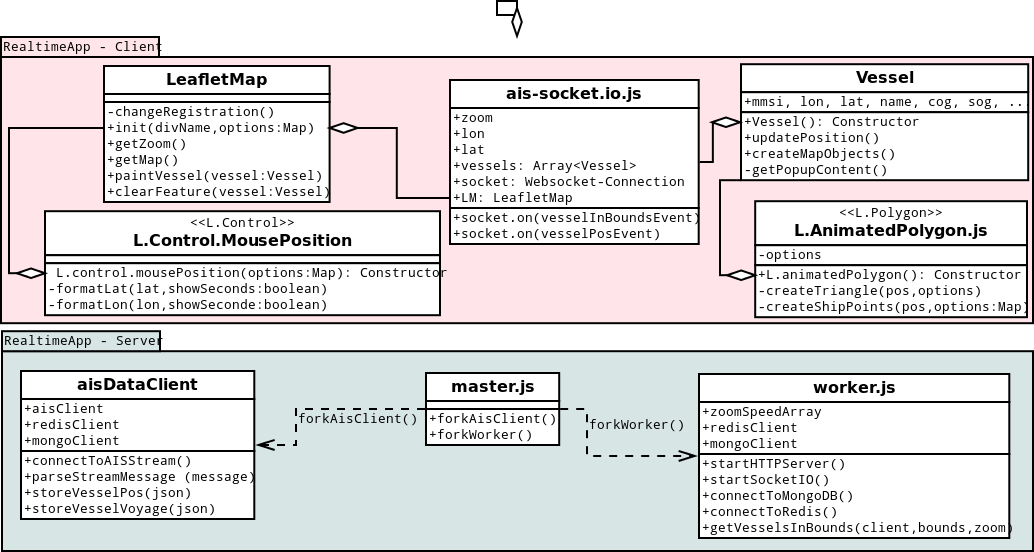
\includegraphics[width=6in]{images/ais-socketio.png}
  \caption[Übersicht Javascript-Files]{Übersicht Javascript-Files}
  \label{fig:Übersicht Javascript-Files}
\end{figure}
\subsection{socket.io-Client}\label{socket.io-Client}
Der socket.io-Client hat folgende Aufgaben.
\begin{enumerate}
\item Es ist eine html-Seite mit den benötigten Bereichen für die Karte zu erstellen.
\item URL-Parameter sollen optional übergeben werden könnenn.
\item Eine Karte mit Navigations- und Infobereichen ist in den Kartenbereich zu rendern.
\item Zum Socket.io-Websocket-Server soll eine Verbindung aufgebaut werden
\begin{itemize}
\item bei Positionsänderungen auf der Karte wird eine register-Nachricht gesendet
\item Vessel-In-Bounds- und Vessel-Position-Events können empfangen werden
\end{itemize}
\item Aus den gesendeten Daten sind geeignete Objekte zu erstellen und zu speichern.
\item Die Objekte sind als Features auf die Karte zu rendern
\item Objekte, die den Status ‘Moving’ haben, sind entsprechend ihrer Geschwindigkeit zu animieren.
\end{enumerate}
Punkt 1 geschieht in der Datei ais-socket.io.html. Dort werden auch die benötigten javascript- und css-Dateien eingebunden. Falls Parameter übergeben werden für Zoomlevel und Bereich werden sie in der javascript-Datei ais-socket.io.js mit der Funktion getParam(name) aufgegriffen.
Als Kartenwerk werden OpenStreetMap-Karten benutzt (siehe Kapitel \ref{OpenStreetMap}). Als Javascript-Bibliothek zur Darstellung der Schiffe auf der Karte fiel die Wahl auf die Leaflet-Bibliotheken. Zwar stützt sich die Cockpit-Anwendug der Vesseltracker-GmbH auf die älteren OpenLayers-Bibliotheken, diese sind jedoch im Vergleich sehr viel sperriger in der Nutzung und werden inzwischen weniger aktiv von der Community weiterentwickelt und verbessert.
Die Karte wird als Javascript-Objekt in der Datei LeafletMap.js realisiert mithilfe des ‘Revealing Module Pattern’. Damit läßt sich die API von der internen Implementierung der Karte trennen. Nur die zurückgegebenen Funktionen bilden die öffentliche Schnittstelle.

\begin{lstlisting}[caption= ‘Revealing Module Pattern’ in LeafletMap.js, label=LeafletMap.js]
var LM = function(){
    var map, featureLayer, tileLayer, zoom, socket, boundsTimeout;
	
    function init(divName, options){...}
    function addOSMLayerToMap(){...}
    function changeRegistration(){...}
    function getMap(){...}
    function getZoom(){...}
    function paintVessel(vessel){...}
    function removePopups(){...}
    function clearFeature(vessel){...}
    
    return {
        init: init,
        getMap: getMap,
        getZoom: getZoom,
        paintVessel: paintVessel,
        clearFeature: clearFeature
    }
}();
\end{lstlisting}

Mit den folgenden Befehlszeilen wird die Websocket-Verbindung hergestellt. Zum Empfang der Nachrichten des Websocket-Servers (siehe Kapitel \ref{socket.io-Server}) genügen zwei Listener: 
\begin{lstlisting}[caption=Client-Seite der socket.io-Websocket-Verbindung in ais-socket.io.js,  label=ais-socket.io.js]
var socket = io.connect('http://127.0.0.1:8090');

socket.on('vesselsInBoundsEvent', function (data) {...}
socket.on('vesselPosEvent', function (data) {...}
\end{lstlisting}

Bezüglich der an den Websocket-Server zu sendenden register-Nachricht ergab sich durch die Kapselung der LeafletMap als revealing Module eine Besonderheit: der moveEnd-Event, der die neue Registrierung triggern soll, befindet sich im LeafletMap-Objekt. Als Lösung wird diese Aufgabe dem LeafletMap-Objekt übertragen, weswegen bei der init-Funktion der socket mit übergeben wird. Diese Lösung ist unproblematisch, weil beim Verlust der socket-Verbindung ohnehin ein Reload der Seite stattfinden muss.
Um geeignete Objekte aus den Ais-Messages zu erstellen (Punkt 5), wird in der Datei Vessel.js eine Konstruktor-Funktion zur Verfügung gestellt, mit der Instanzen von Vessel-Objekten generiert werden können. Diese Instanzen werden in einem assoziativen Array, also einem Objekt, namens ‘vessels’ gespeichert. Beim Empfang eines Vessel-Position-Events kann mit vessels[mmsi] nach dem passenden vessel-Objekt zum Update gesucht werden.
Schließlich sind die Vessel-Objekte auf die Karte zu rendern. Dazu wird in Vessel.js eine asynchrone Funktion genutzt (siehe Listing \ref{vessel.createMapObjects}), mit der zuerst je nach Status (moving / not moving) und zoomlevel unterschiedliche Features für ein Schiff erstellt werden (Polygon, Triangle, Speedvector, Circle). Anschließend wird das vessel-Objekt auf die Karte gerendert und das Objekt mit den Features gespeichert. Das ist notwendig, um die Features bei Vessel-Position-Updates von der Karte zu entfernen, bevor sie an der neuen Position dargestellt werden.
\begin{lstlisting}[caption=Aufruf der public function createMapObjects des Vessel-Objekts in ais-socket.io.js, label=vessel.createMapObjects]
vessel.createMapObjects(LM.getZoom(), function(){
              LM.paintVessel(vessel);
              vessels[vessel.mmsi] = vessel;
            });
\end{lstlisting}

Für díe letzte Aufgabe, die Animation, wird das Polygon-Objekt des Leaflet-Frameworks erweitert zur Klasse L.AnimatedPolygon. Ein Polygon in Leaflet ist eine Polyline, die mehrere Punkte auf der Karte verbindet. Die Animation eines Punktes entlang einer Linie mit einer bestimmten Geschwindigkeit wurde aus dem Leaflet-Plugin L.AnimatedMarker \footnote{\label{foot:2}https://github.com/openplans/Leaflet.AnimatedMarker} übernommen. Die dort präferierte css3-Transition zur Animation konnte aber nicht verwendet werden, weil dazu ein Objekt im DOM-Baum verwendet werden muss. Das von Leaflet für ein Polygon erstellte DOM-Objekt (svn-Graphik) ist aber durch die Leaflet-Bibliothek gekapselt, so dass ein Zugriff von außen nicht vorgesehen ist.  \\

Ein Schiffspolygon wird berechnet aus der Schiffsposition (Positionsangabe in der AIS-Nachricht) und aus der relativen Position des AIS-Transceivers an Bord (Abstand zum Bug, zum Heck, nach Backbord und nach Steuerbord). Um zu wissen, in welche Richtung der Bug eines Schiffes zeigt, wird die AIS-Angabe zur Fahrtrichtung (cog = Course over Ground) verwendet. Aus dieser Richtungsangabe und der übermittelten Geschwindigkeit (sog = Speed over Ground) wird ein Speedvector berechnet, der als Linie auf die Karte gezeichnet wird. Bei der Erstellung des AnimatedPolygon-Objektes wird dieser Speedvector mit übergeben, um bei der Animation des Polygons die Position des Schiffes entlang des Speedvektors zu verschieben. Nach jedem Animationsschritt wird das Polygon neu berechnet und gezeichnet.


\subsection{HTML5-Server}\label{HTML5-Server}
Diese Server-Implementierung soll genau dieselbe Funktionalität besitzen wie die socket.io-Server-Implementierung (\ref{socket.io-Server}). Lediglich der Websocket socket.io wird durch einen node.js-Websocket nach der HTML5-Websocket-Spezifikation ausgetauscht \footnote{\label{foot:2}https://github.com/Worlize/WebSocket-Node} . Dazu wird in der Datei worker.js das entsprechende Paket (‘websocket’) eingebunden.
Einige Features des socket.io-Paketes müssen jetzt selbst organisiert werden: 
\begin{itemize}
\item die Clientverwaltung erfolgt in einem Array ‘clients’, in dem zu jeder Zeit alle verbundenen Clients mit ihren Attributen stehen. 
\item in der Websocket können keine eigenen Events definiert werden (siehe API-Dokumentation \footnote{\label{foot:2}https://github.com/Worlize/WebSocket-Node/wiki/Documentation}. Deshalb wird der message-Event genutzt und die aufzurufende Funktion wird in der message übermittelt.
\end{itemize}
\begin{lstlisting}[caption= vom Websocket-Server gesendete message, label=websocket-message]
message origin=ws://127.0.0.1:8090, data={"type":"vesselsInBoundsEvent","vessels":[{"_id":"50d9fdb4bcc2e678a9278c18","aisclient_id":57,"callsign":"OVYC2 ","cog":285,"dest":"HAMBURG ","dim_bow":70,"dim_port":10,"dim_starboard":4,"dim_stern":30,"draught":54,"imo":"9363170","mmsi":220515000,"msgid":1,"name":"RIKKE THERESA ","nav_status":0,"pos":[9.85185,53.54643333333333],"rot":0,"ship_type":80,"sog":10.3,"time_captured":1366733896000,"time_received":1366733855248,"true_heading":286}]}

\end{lstlisting}
\begin{lstlisting}[caption= vom socket.io-Server gesendete message, label=socket.io-message]
[{"_id":"50d9fdb4bcc2e678a9278c18","aisclient_id":57,"callsign":"OVYC2  ","cog":286,"dest":"HAMBURG             ","dim_bow":70,"dim_port":10,"dim_starboard":4,"dim_stern":30,"draught":54,"imo":"9363170","mmsi":220515000,"msgid":1,"name":"RIKKE THERESA       ","nav_status":0,"pos":[9.8375,53.54885],"rot":0,"ship_type":80,"sog":12.4,"time_captured":1366734056000,"time_received":1366734014715,"true_heading":288}]
\end{lstlisting}

\subsection{HTML5-Client in Javascript}\label{HTML5-Client in Javascript}
Die socket.io-Client-Implementierung und die HTML5-Client bieten die gleiche Funktionalität und arbeiten nur geringfügig unterschiedlich.
 \begin{itemize}
 \item wie inListing \ref{socket.io-message} und \ref{websocket-message} zu sehen, muss der HTML5-Client zuerst den message-type abfragen, um die Daten korrekt zuzuordnen.
 \item weil dem Leaflet-Map-Objekt die Websocket-Connection als Parameter übergeben wird, muss dafür der Aufbau der Websocket-Connection abgewartet werden. 
\end{itemize}

\subsection{HTML5-Client in Dart}\label{HTML5-Client in Dart}
Die Implementierung des HTML5-Client in Dart orientiert sich an der Implementierung des HTML5-Websocket-Clients in Javascript. Oberstes Ziel dabei ist es, dieselbe Funktionalität zu implementieren wie in \ref{HTML5-Client in Javascript} unter Ausnutzung der sprachspezifischen Vorteile. \\

Die Modularisierung, also die Verteilung der Objekte und Funktionalitäten auf Programmdateien, ist in der Dart-Client-Implementierung ähnlich gestaltet wie in Javascript (siehe Abb. \ref{fig:Übersicht Javascript-Files}). Die verwendeten Javascript-Dateien (Leaflet-Bibliothek, L.AnimatedPolygon, L.Control.Mouseposition) sind identisch mit denen in \ref{HTML5-Client in Javascript}. Um sie aus Dart heraus nutzen zu können, wird das Dart-Paket js-interop (\ref{js-interop}) eingebunden.

Die main-Funktion in ais-html5.dart startet die Anwendung, die den html5-Websocket initialisiert. Im Falle eines erfolgreichen Verbindungsaufbaus wird die Callback-Funktion ausgeführt, die das LeafletMap-Objekt erstellt. Beide Objekte sind Singletons und bleiben über die Laufzeit der Anwendung erhalten.
Das LeafletMap-Objekt kapselt für die Anwendung den Zugriff auf das javascript L.Map-Objekt der leaflet.js-Bibliothek (siehe Listing \ref{LeafletMapConstructor}). Dafür wechselt es in den Javascript-Scope der Anwendung und initialisiert in diesem ein L.Map-Objekt und ein L.LayerGroup-Objekt und deklariert sie mit der Anweisung js.retain(...) im javascript-Scope als globale Variable, so dass sie für jede folgende Funktion, die den javascript-Scope benutzt, zur Verfügung stehen.
In der Gegenrichtung muss eine Möglichkeit existieren, von der Javascript-Seite der Anwendung den Dart-Code aufzurufen. Ein Beispiel dafür ist der moveend-Listener, der Teil der leaflet.js-Bibliothek ist. Für den Javascript-Listener wird ein Dart-Callback.many-Objekt aus der Dart-Funktion changeRegistration() erstellt. Das Dart-Callback.many-Objekt kann im Unterschied zum Callback.once-Objekt mehrmals aufgerufen werden. Das heißt, jedes Mal, wenn in Javascript der Moveend-Listener einen Moveend-Event registriert, ruft er die Dart-Funktion changeRegistration auf. Diese Funktion sendet an den HTML5-Websocket eine Nachricht vom Typ ‘register’ mit den aktuellen Bounds der Karte.

\begin{lstlisting}[caption=Konstruktor des LeafletMap-Objektes mit Zugriff auf den javascript-Scope, label=LeafletMapConstructor]
LeafletMap(String elementid, js.Proxy mapOptions,  js.Proxy initOptions, js.Proxy tileLayerOptions){
    boundsTimeout = initOptions['boundsTimeout']*1000;
    js.scoped(() {
        map = new js.Proxy(js.context.L.Map, elementid, mapOptions);
        featureLayerGroup = new js.Proxy(js.context.L.LayerGroup);
        map.addLayer(featureLayerGroup);
        js.retain(featureLayerGroup);
        var osm = new js.Proxy(js.context.L.TileLayer,tileLayerOptions['tileURL'], tileLayerOptions);
        map.addLayer(osm);
        var mouseOptions = js.map({'numDigits': 5  });
        if(initOptions['mousePosition'] == true)
        {
          var mouseOptions = js.map({'numDigits': 5  });
          var mousePosition = new js.Proxy(js.context.L.Control.MousePosition, mouseOptions);
          mousePosition.addTo(map);
        }
        map.setView(new js.Proxy(js.context.L.LatLng, initOptions['lat'], initOptions['lon']),initOptions['zoom']);
        js.retain(map);
        map.on('moveend', new js.Callback.many(moveendHandler));
      });
    changeRegistration();
  }
\end{lstlisting}
Der Websocket-Server antwortet auf diese Nachricht mit einer Nachricht von Typ “VesselInBoundsEvent” (siehe Listing \ref{websocket-message}).

Ebenso kapselt die eigene Bibliothek MapFeature.dart den Zugriff auf die L.Feature-Objekte der leaflet.js-Bibliothek. 
So kann der moveend-Event, der nach dem Rendern der Karte ausgelöst wird, über die changeRegistration-Funktion und den bereitgestellten websocket den ersten Vessel-In-Bounds-Request senden.



, die die beiden Dart-Libraries Vessel (Vessel.dart) und LMap (LeafletMap.dart) einbindet. Die Library Vessel stellt die Klasse Vessel für die Initialisierung der Vessel-Objekte zur Verfügung, die Library leaflet\_map stellt die abstrakte Klasse LeafletMap zur Verfügung mit ihrer konkreten Ausprägung OpenStreetMap 


%--------------------------------------------------------------------------------------------------------------------------------------------

\chapter{Ergebnisse}\label{Ergebnisse}

\section{Evaluation der Anwendung}\label{Evaluation der Anwendung}
\subsection{Funktionale Anforderungen}
Alle funktionalen Anforderungen aus Abschnitt \ref{s.Beschreibung der Anforderungen} sind im Prototyp der Anwendung in Javascript mit dem node.js-Framework und dem socket.io-Websocket-Server aus Abschnitt \ref{socket.io-Server} und -Client aus Abschnitt \ref{socket.io-Client}) vollständig umgesetzt. Im Screenshot des Hamburger Hafens (Abb. \ref{Hafen Hamburg}) kann man erkennen, dass liegende Schiffe als Kreise dargestellt werden und fahrende Schiffe als Richtungsdreiecke. Wurden Reisedaten zu einem Schiff übermittelt (AIS-Nachricht vom Typ 4), sind maßstabsgetreue Polygone eingezeichnet, deren Farbe den Schiffstyp kennzeichnet.
Ein Popup mit Detailinformationen zum dem Schiff links daneben ist geöffnet. In dieser Zoomstufe ist die Animation bereits aktiv, das heißt für den Betrachter, dass alle angezeigten Richtungsdreiecke sich ihrer tatsächlich Geschwindigkeit angemessen bewegen.

\begin {figure}[H]
\begin{center}
  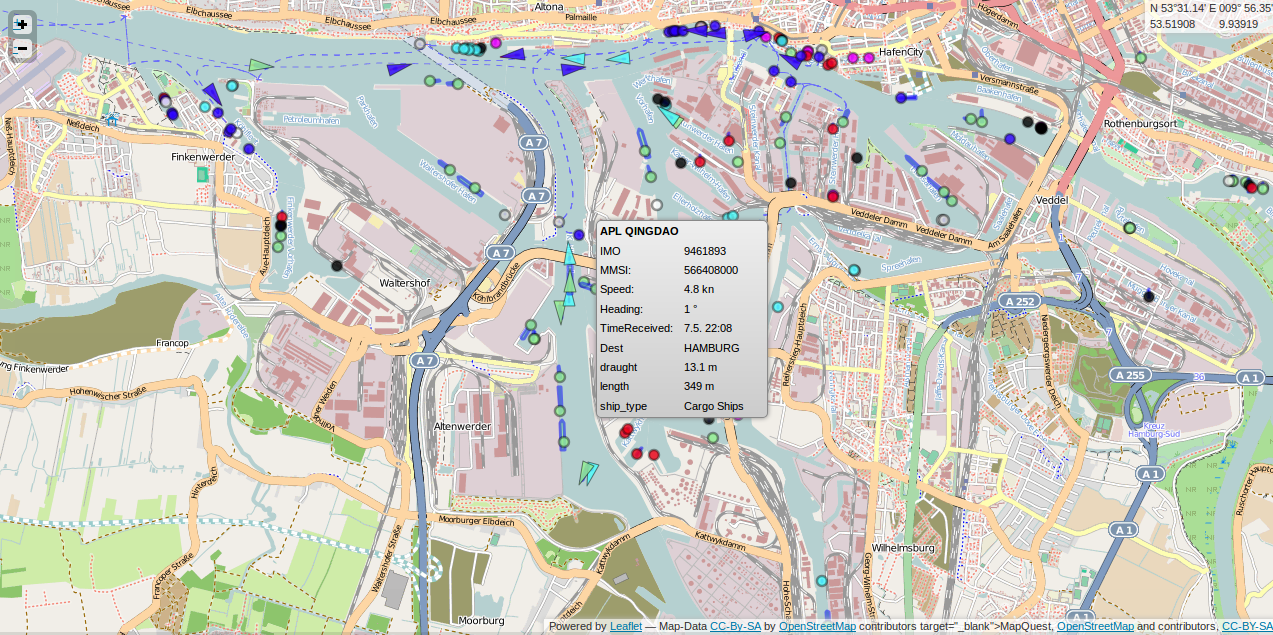
\includegraphics[width=6in]{images/Hamburg.png}
\end{center}
\caption{Anzeige aller Schiffe im Hamburger Hafen}
\label{Hafen Hamburg}
\end {figure}
Abbildung \ref{Nordsee} zeigt die Situation bei niedriger Zoomstufe. Links oben in der Karte ist der Hinweis eingeblendet, dass nur Schiffe mit einer Geschwindigkeit über 12 Knoten angezeigt werden. Die Verteilung des Schiffsverkehrs lässt sich gut erkennen, während die große Zahl hafenliegender Schiffe aus Perfomancegründen ausgespart bleibt. Aus demselben Grund ist die Animation ausgeschaltet. Durch die hohe Frequenz empfangener Positionsmeldungen ist die Darstellung trotzdem in Bewegung.

\begin {figure}[H]
\begin{center}
  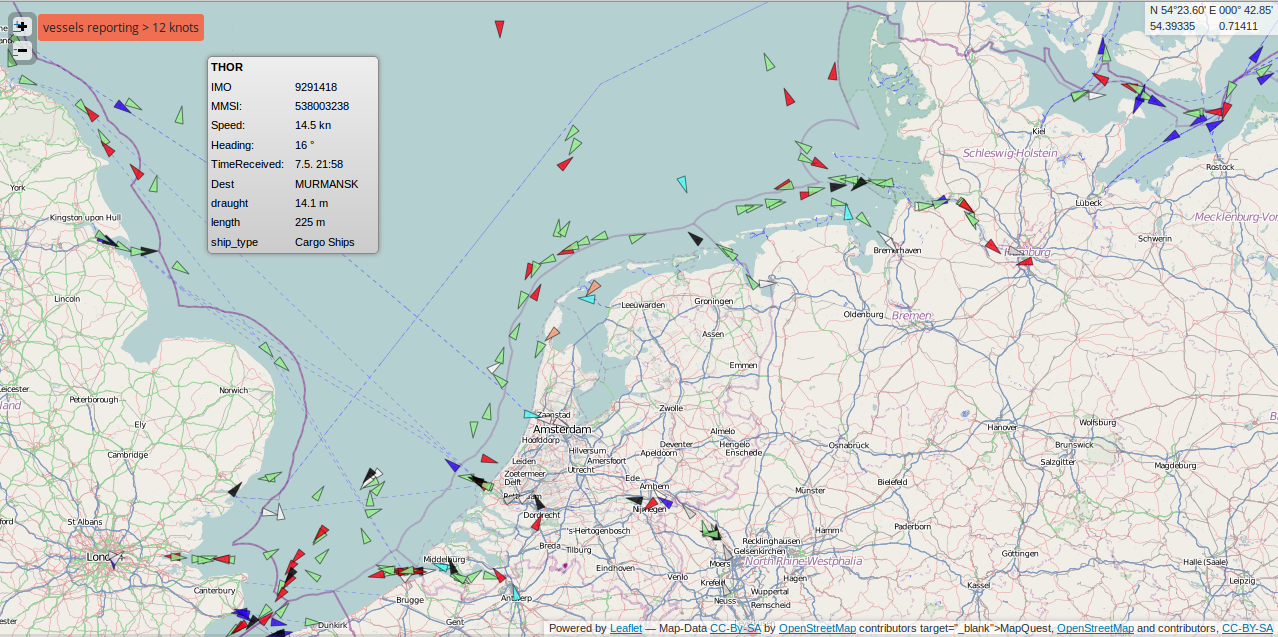
\includegraphics[width=6in]{images/zoomout.png}
\end{center}
\caption{Auf schnell fahrende Schiffe reduzierte Anzeige am Beispiel der Nordsee}
\label{Nordsee}
\end {figure}

\begin {wrapfigure}[9]{r}{3in}
\begin{center}
  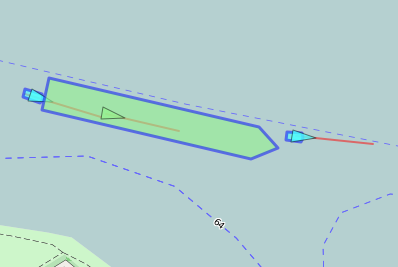
\includegraphics[width=2in]{images/Schleppen.png}
 \caption{Schleppmanöver}
  \end{center}
 \label{Schleppmanöver}

\end {wrapfigure}

Schließlich ist in hohen Zoomstufen eine Beobachtung von aktuellen Schiffsmanövern möglich, wie in Abbildung \ref{Schleppmanöver} das Schleppen eines Frachtschiffes durch zwei Schleppschiffe. Die hohe Frequenz der Positions-Meldungen bei fahrenden Schiffe und die eingebaute Animation lassen den Betrachter die Szene wie in einem Animationsfilm erleben.\\
\subsection{Nicht funktionale Anforderungen}
Die vorgestellte Implementierung erfüllt auch die wichtige nicht funktionale Anforderung nach einer zeitnahen Umsetzung. Sie wurde Ende Februar 2013 an das Unternehmen Vesseltracker übergeben und wird auf github als privates Repository gehostet.
Die gesamte Anwendung ist mit open source Produkten entwickelt worden und verwendet das von der Vesseltracker gehostete OpenstreetMap-Kartenmaterial.\newline
Die Anwendung wurde auf den unten angegebenen Browserclients in den angegebenen Versionen positiv auf Funktionalität getestet und unterstützt damit die gängen Browser in den einschlägigen Versionen \footnote{http://www.browser-statistik.de/statistiken/versionen/}:
\begin{itemize}
\item Firefox Version 15.0.1 und 20.0
\item Google Chrome 26.0
\item Internet Explorer Version 9.0 und 10.0
\item Safari 6.0.4
\end {itemize}

Die Latenzzeit zwischen dem Empfang der AIS-Positions-Meldung durch den Rohdatenserver und der Propagierung derselben Position auf der Karte sollte unterhalb 500 msec liegen. Hier sei verwiesen auf die Ergebnisse in Abschnitt \ref{socket.io- vs html5-Server} und Abbildung \ref{Latenzzeit socket.io}. Die gemessenen Latenzzeiten liegen vollständig innerhalb der geforderten Geschwindigkeit.


Die Anzahl der Verbindungen, die der Server gleichzeitig bedienen kann, ist mit einem node.js-Script getestet worden, das alle 500 ms eine neue Clientverbindung erstellt bis 750 Clients verbunden sind. Der Aufbau der Verbindung geschah auch mit steigender Verbindungsanzahl zuverlässig, jedoch ist in Abbildung \ref{Antwortzeiten socket.io} erkennbar, dass die Anzahl der Fälle zunimmt, in denen ein Client lange auf Antwort warten muss.
\\Eine Skalierung der Serveranwendung ist seitens des socket.io-Servers kein Problem. Statt einen einzigen Worker-Prozess zu generieren, können auch mehrere Worker-Prozesse parallel gestartet werden, die alle dieselbe mongo-Datenbank-Collection abfragen und sich bei derselben redis-Datenbank im Channel ‘positionUpdate’ registrieren können. Allerdings muss sichergestellt sein, z.B.  über unterschiedliche Ports oder unterschiedliche (virtuelle) Server, dass ein verbundener Client mit jedem neuen Request auf demselben Worker-Prozess landet.

\begin{figure}[H]
\begin{minipage}[hbt]{3in}
	\centering
	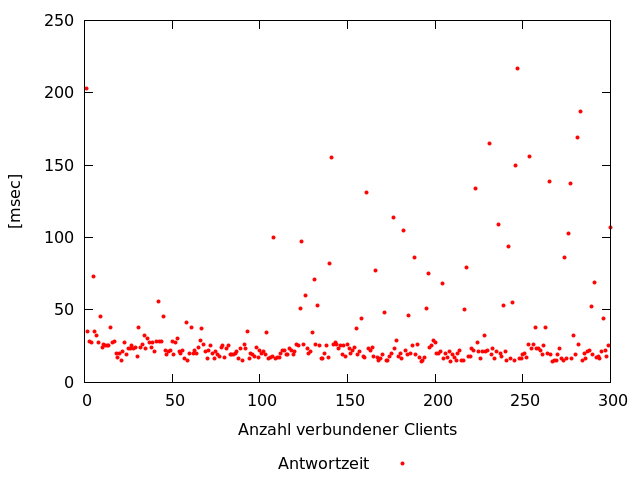
\includegraphics[width=2.5in]{images/stresstest300.png}
	\label{Stresstest300}
\end{minipage}
\hfill
\begin{minipage}[hbt]{3in}
	\centering
	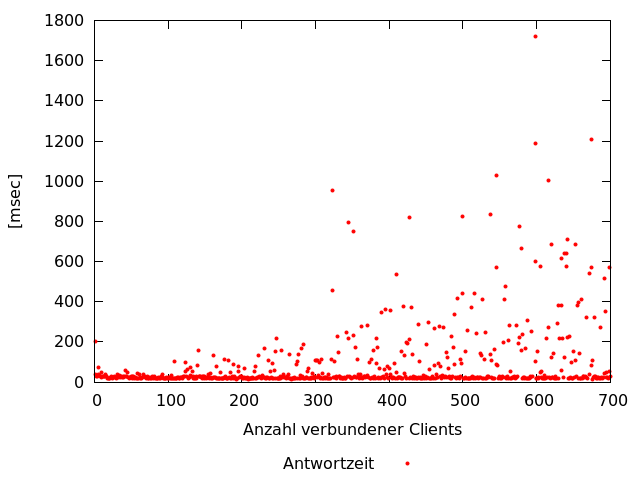
\includegraphics[width=2.5in]{images/stresstest.png}
	\label{Stresstest}
\end{minipage}
\caption{Anwortzeiten des socket.io-Websocket-Servers in Abhängigkeit von der Anzahl verbundener Clients}
\label{Antwortzeiten socket.io}
\end{figure}
%-------------------------------------------------------------------------------------------------------------------------------------------
\section{Vergleichende Evaluation der Javascript- und der Dart-Anwendung}
Für alle folgenden Tests wird auf dem Rohdatenserver ein Port eingerichtet, der nur die Daten von drei AIS-Antennen (Hamburg, Wedel, Geesthacht) als Datenstrom ausgibt. Dies ist notwendig, weil der als Server (und Client) verwendete Arbeitsplatzrechner (HP 530 Notebook PC mit 1,8 GHz Intel Celeron Processor und 1,5 GB Arbeitsspeicher) die Datenmenge aller AIS-Meldungen weltweit nicht in der Geschwindigkeit verarbeiten kann, in der sie eingehen. Dadurch wächst die Messagequeue des Node.js-Servers und erzeugt eine zusätzliche Latenzzeit, die die Ergebnisse verzerrt.

Die in den Abschnitten  \ref{Strategie-Korrektur} und \ref{Vergleichbarkeit} begründete zusätzliche Implementierung eines HTML5-kompatiblen node.js-Websocket-Servers muss nun in einem ersten Schritt mit dem node.js-socket.io-Server verglichen werden. Anschließend wird die in Google Dart geschriebene Client-Anwendung mit dem in Javascript programmierten Client verglichen.
%-------------------------------------------------------------------------------------------------------------------------------------------
\subsection{Vergleich des socket.io-Servers mit dem HTML5-Server}\label{socket.io- vs html5-Server}
\subsubsection{Implementierungsaufwand}
Im Implementierungsaufwand unterscheiden sich beide Server- und Client-Anwendungen kaum. Die Unterschiede in Zeilen Code betragen weniger als 10 Zeilen.\\
Einige Features der socket.io-Bibliotheken (z.B. die Clientverwaltung, Parameter für ‘Production’ und ‘Development’-Umgebung bezüglich Log-Leveln, Client-Minifikation oder Client-Zip) sind praktisch und müssten in der Alternativimplementierung für den Einsatz in einer Produktiv-Umgebung anderweitig gelöst werden. Durch die in socket.io eingeführten Events vermindert sich der Kommunikationsaufwand zwischen Server und Client geringfügig, was in diesem Fall einer datenintensiven Anwendung mit großen Datenmengen pro Nachricht kaum ins Gewicht fällt.
\subsubsection{Latenzzeit}
Die Leistungsfähigkeit beider Implementierungen wird verglichen, indem die Zeit gemessen wird, die eine Positionsmeldung braucht für den Weg vom Rohdatenserver bis zur Präsentation auf der Karte.
Auf dem Rohdatenserver wird jeder AIS-Message beim Empfang ein Zeitstempel (time\_received) hinzugefügt. Dazu läuft auf dem Rohdatenserver ein ntp-Daemon zur Zeitsynchronisation. Genau so ein Daemon läuft auf dem Client, auf dem der Browser gestartet wird. Ein Zeitstempel wird genommen, nachdem das Schiff mit der neuen Position auf die Karte gerendert wurde. Die Latenzzeit berechnet sich dann aus der Differenz zwischen der time\_received und diesem Zeitstempel. \\
Um eine ähnliche Situation in beiden Szenarien abzubilden, wird jeweils eine bestimmte Position im Hamburger Hafen mit maximaler Zoomstufe angesteuert und ein Timer in die Client-Anwendungen integriert, der jeweils nach einer Minute um eine Stufe herauszoomt. Da ab Zoomlevel 11 und kleiner nur noch Schiffe mit einer jeweils definierten Mindestgeschwindigkeit angefordert werden, nimmt die Anzahl empfangener Schiffe von dieser Zoomstufe an wieder ab. Zur Auswertung wird auf dem Client ein LogFile geschrieben, das für jede Positionsmeldung deren ‘time\_received’ und einen aktuellen Zeitstempel festhält. Die Differenz wird als Latenzzeit interpretiert. Anschließend wird über das Logfile berechnet, wieviele Positionsmeldungen in einer Minute an den Client gesendet wurden. In den Abbildungen \ref{Latenzzeit socket.io} und \ref{Latenzzeit HTML5} sind jeweils beide Ergebnisse über die Zeit der Beobachtung (ca. 15 min) aufgetragen.
\begin {figure}[H]
\begin{center}
  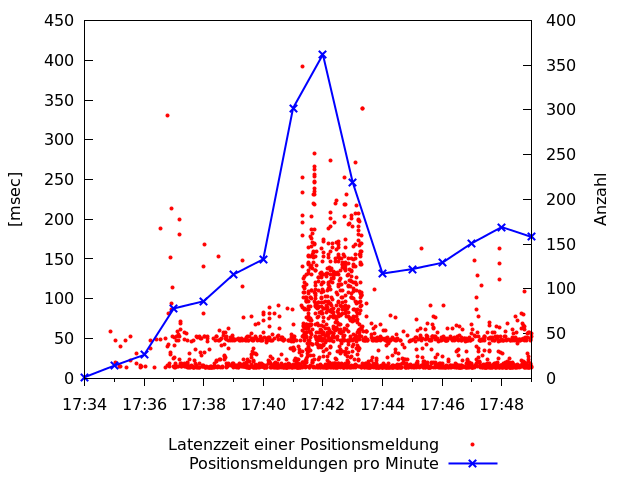
\includegraphics[width=4.5in]{images/latency_timeReceived_socket_io.png}
\end{center}
\caption{socket.io-Websocket-Server: Latenzzeit der Positionsmeldungen und Anzahl empfangener Schiffe}
\label {Latenzzeit socket.io}
\end {figure}

\begin {figure}[H]
\begin{center}
  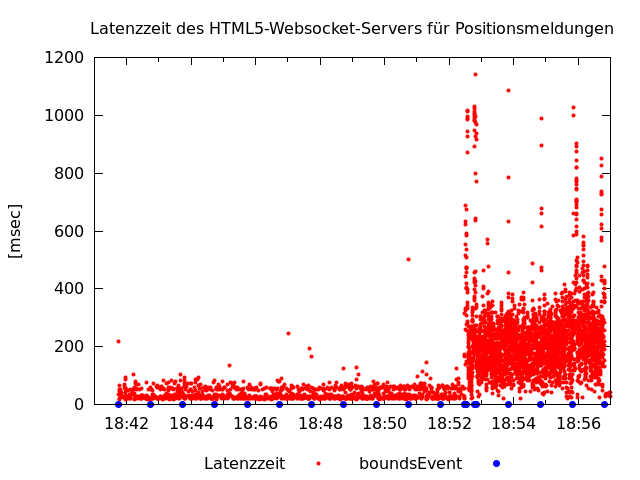
\includegraphics[width=4.5in]{images/latency_timeReceived_HTML5.png}
\end{center}
\caption{HTML5-Websocket-Server: Latenzzeit der Positionsmeldungen und Anzahl empfangener Schiffe}
\label {Latenzzeit HTML5}
\end {figure}
Es ist offensichtlich, dass die Geschwindigkeit in der Darstellung von der Anzahl empfangener Nachrichten linear abhängt.Darüber hinaus ist zu erkennen, dass beide Implementierungen ihre Aufgabe in vergleichbarer Geschwindigkeit erledigen. 
Das bedeutet, dass die HTML5-Node.js-Anwendung in ihrer Leistungsfähigkeit der socket.io-Node.js-Anwendung gleichwertig ist und im Folgenden als repräsentative Javascript-Lösung verwendet werden kann.

\subsubsection{Browserunterstützung}
Für die  node.js-HTML5-Websocket-Anwendung wird wie für die socket.io-Websocket-Anwendung in Abschnitt \ref{Evaluation der Anwendung} die Unterstützung durch die gängigen Browser getestet (Tabelle \ref{Browserclients-Vergleich}).

\begin{table}[H]
\begin{center}
\small
\texttt{
\begin{tabular}{ l|r|c|c}
\bf{Browser}&\bf{Version}&\bf{socket.io}&\bf{HTML5}\\\hline
Firefox& 20.0&websocket&websocket \\
Google Chrome & 26.0 &websocket&websocket\\
Internet Explorer&9& Flashsocket&nicht unterstützt\\
Internet Explorer&10& websocket&websocket\\
Safari&6.0.4 & websocket&websocket\\
\end{tabular}
}
\end{center}
\caption[Unterstützung von Browsern durch die socket.io- und HTML5-Websocket-Clients]{Unterstützung von Browsern durch die socket.io- und HTML5-Websocket-Clients}
\label{Browserclients-Vergleich}
\end{table}

Erwartungsgemäß unterstützen alle gängigen aktuellen Browser HTML5-kompatible Websockets\footnote{http://caniuse.com/\#search=websocket}. Für ältere Browser ohne Websocket-Unterstützung wie den IE 9 bietet socket.io einen Fallback auf Adobe Flashsocket. Listing \ref{flashsocket} zeigt den Client-Request des socket.io-Clients im IE 9, der vom Server den Flashsocket (WebSocketMain.swf) anfordert. In der HTML5-Anwendung dagegen beendet der IE 9  mit einem Scriptfehler die Anwendung.\\
\begin{lstlisting}[language=html,caption=socket.io Client-Request in Internet Explorer 9, label=flashsocket]
Anforderung     GET /socket.io/static/flashsocket/WebSocketMain.swf HTTP/1.1
Accept  */*
Accept-Language de-DE
Referer http://192.168.1.214:8090/ais-socket.io_js.html
x-flash-version 10,0,32,18
Accept-Encoding gzip, deflate
User-Agent      Mozilla/5.0 (compatible; MSIE 9.0; Windows NT 6.1; Trident/5.0)
Host    192.168.1.214:8090                            
\end{lstlisting}

%-----------------------------------------------------------------------------------------------------------------------------------------------
\newpage
\subsection{Vergleich des Javascript-Clients mit dem Dart-Client} 
\subsubsection{Implementierungsaufwand}
Die Möglichkeit des objektorientierten Programmierens in Dart bringt beim Implementieren des Dart-Clients die größte Erleichterung gegenüber der Implementierung in Javascript. Die geschaffene Struktur ist in Abbildung \ref{fig:Übersicht Dart-Files} zu erkennen. Javascript bietet zwar zahlreiche Lösungen, um Objektorientierung nachzubilden, z.B. über Funktionen als Klassen-Objekte und Konstrukte wie das Revealing Module Pattern. Dadurch wird das Programmieren in Javascript aber mit zunehmender Komplexität der Anwendung unübersichtlicher und fehleranfälliger, weil die Features objektorientierter Sprachen sozusagen per Hand gepflegt werden müssen. Die entstehenden Strukturen sind weniger transparent und selbsterklärend als in Dart (\ref{fig:Übersicht Javascript-Files}).
\begin {wraptable}{r}{2in}
\begin{center}
\small
\texttt{
\begin{tabular}{ l|c}
Client&Zeilen Code\\\hline
Javascript& 611 \\
Dart& 867\\
\end{tabular}
}
\caption[Anzahl Zeilen Code im Vergleich der Clients]{Anzahl Zeilen Code im Vergleich der Clients}
\label{Zeilen Code}
\end{center}
\end{wraptable}
Die Dart-Implementierung der Anwendung wird an dem Punkt etwas aufwändiger, wo über das Paket js-interop die Javascript-Dateien integriert werden und Proxies und Callback-Funktionen geschrieben werden müssen zur Kommunikation zwischen dem Javascript- und dem Dart-Kontext. Der quantitative Mehraufwand spiegelt sich auch in einem signifikanten Unterschied in der Anzahl Zeilen Code (Tabelle \ref{Zeilen Code}).\\
Mit dem dart2js-Compiler ließ sich der Dart-Client-Code zu Javascript kompilieren und war dann auch auf Browsern ohne Dart VM ausführbar. Dabei traten gelegentlich Fehler auf, die entweder auf Bugs zurückzuführen waren und mit dem nächsten Update behoben waren oder Fehler, die durch Änderungen im Dart-Code behoben werden mussten, obwohl der originäre Dart-Code von der Dart VM korrekt interpretiert wurde. Dazu ein Beispiel:\\
Wird innerhalb des Javascript-Kontexts eine Methode auf einen Javascript-Proxy (hier \_map) aufgerufen und ein Javascript-Proxy wird zurückgegeben, dann ist es möglich, auf diesen Proxy, der in diesem Fall vom Typ LatLngBounds ist, eine Methode der Klasse LatLngBounds aufzurufen (siehe Listing \ref{LeafletMap.dart}). Im zu Javascript kompilierten Dart-Code lief die Anwendung damit jedoch in einen Fehler:\\
“=> TypeError: t1.get\$\_map(...).getBounds\$0(...).getSouthWest\$0 is not a function”\\

\begin{lstlisting}[caption= LeafletMap.dart mit ursprünglicher Abfrage des Bounds-Objektes, label= LeafletMap.dart]
  List getBounds(){
    var south, west, north, east;
    js.scoped((){
    south= _map.getBounds().getSouthWest().lng;
        west = _map.getBounds().getSouthWest().lat;
        north = _map.getBounds().getNorthEast().lng;
        east = _map.getBounds().getNorthEast().lat;
 });
return [west, south, east, north];
}

 changeRegistration(){
    int zoom = getZoom();
    var boundsList = getBounds();
    Map _southWest = {"lng":boundsList[0],"lat":boundsList[1]};
    Map _northEast= {"lng":boundsList[2],"lat":boundsList[3]};
    Map bounds = {"_southWest": _southWest,"_northEast":_northEast};

    Map message = new Map();
    message['function'] = 'register';
    message['zoom'] =  zoom;
    message['bounds'] = bounds;
    socket.send(stringify(message));
    
    boundsTimeoutTimer = new Timer(new Duration(milliseconds:boundsTimeout),changeRegistration);  
  }
\end{lstlisting}
Weil kein Bug zu diesem Problem über die Dart-Communiy\footnote{https://www.dartlang.org/community/} zu finden ist, wird das Problem mit einem Workaround behoben. Und zwar wird über die Methode ‘getBBoxString’ des Bounds-Objekt ein String mit den Bounds geholt. Aus diesem String sind anschließend die Double-Werte für die Bounds zu parsen (Listing \ref{LeafletMap.dart mit workaround}).
\begin{lstlisting}[caption= LeafletMap.dart mit workaround über BBoxString, label= LeafletMap.dart mit workaround]
String getBounds(){
    String bBox;
    js.scoped((){
      bBox = \_map.getBounds().toBBoxString();
    });
    return bBox;
  }
  changeRegistration(){
    int zoom = getZoom();
    var boundsArray = getBounds().split(",");
    Map _southWest = {"lng":double.parse(boundsArray[0]),"lat":double.parse(boundsArray[1])};
    Map _northEast= {"lng":double.parse(boundsArray[2]),"lat":double.parse(boundsArray[3])};
    Map bounds = {"_southWest": _southWest,"_northEast":_northEast};
    Map message = new Map();
    message['function'] = 'register';
    message['zoom'] =  zoom;
    message['bounds'] = bounds;
    socket.send(stringify(message));
      boundsTimeoutTimer = new Timer(new Duration(milliseconds:boundsTimeout),changeRegistration);  
  }
\end{lstlisting}

\subsubsection{Performance}
Um die Performance des Javascript-Clients mit der des eigentlichen Dart-Clients und des zu Javascript kompilierten Dart-Clients zu vergleichen, wurde der VesselsInBounds-Event genutzt. Gemessen wurde die Zeit, die benötigt wird, um nach Empfang eines VesselInBounds-Events alle in der Message enthaltenen Schiffe auf die Karte zu rendern. Verglichen wurden die Clients in den Browsern Dartium, Chrome und Firefox.
\begin{itemize}
\item Google Dartium interpretiert den originären Dart-Client mit der Dart VM. Beim Aufruf des Javascript-Clients in Dartium wird der Javascript-Code mit der V8-Javascript-Engine interpretiert.
\item Google Chrome  mit der V8-Javascript-Engine führt beim Aufruf des Dart-Clients den zu javascript kompilierten Dart-Code aus und beim Aufruf des Javascript-Clients den originären Javascript-Code.
\item ebenso führt Firefox mit der SpiderMonkey Javascript Engine den zu Javascript kompilierten Dart-Client-Code, bzw. den originären Javascript-Client-Code aus.
\end {itemize}
%\newpage
In einer ersten Testserie wurden die Browserclients auf dem HP 530 Notebook PC mit 1,8 GHz Intel Celeron Processor und 1,5 GB Arbeitsspeicher ausgeführt, auf dem auch die Server-Anwendung läuft.

\begin {figure}[H]
\begin{center}
  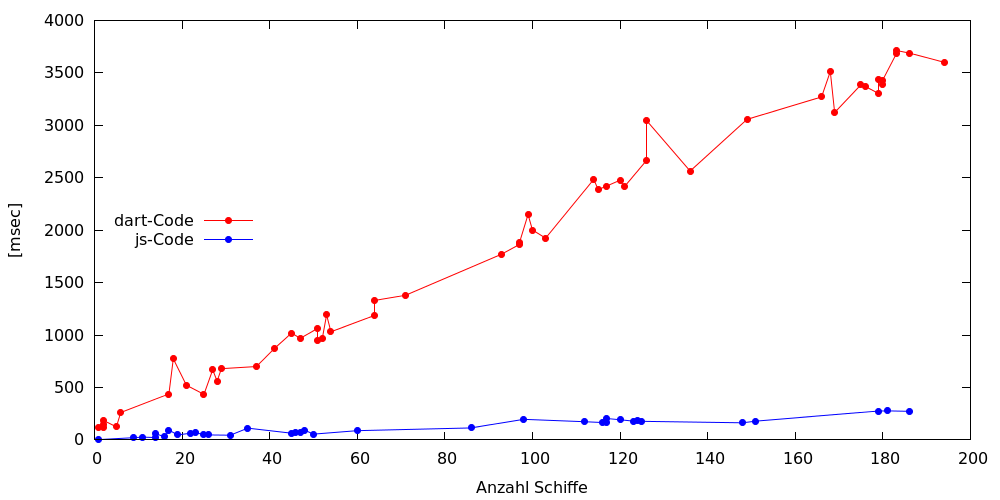
\includegraphics[height=2.3in]{images/Dartium.png}
\end{center}
 \caption{Verarbeitungsdauer in Dartium (HP 530 Notebook PC)}
\end {figure}


\begin {figure}[H]
\begin{center}
  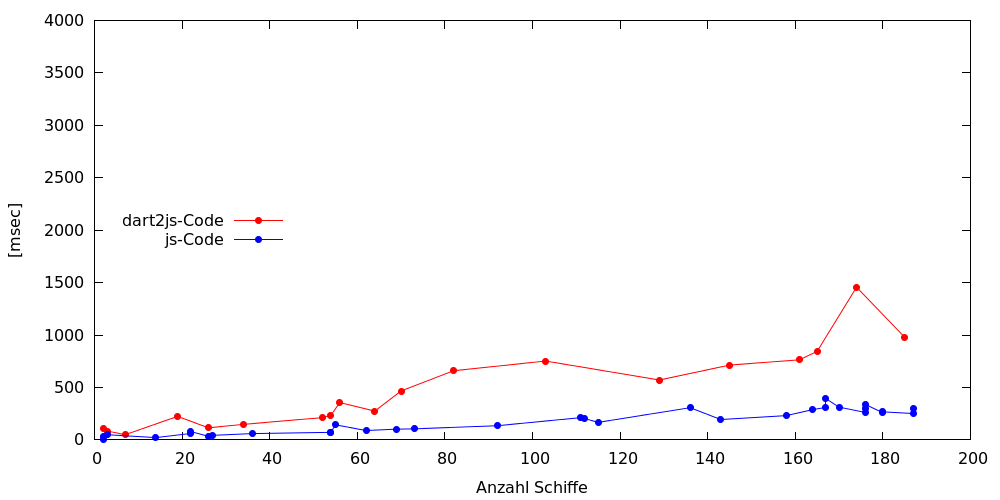
\includegraphics[height=2.3in]{images/Chrome.png}
\end{center}
 \caption{Verarbeitungsdauer in Chrome (HP 530 Notebook PC)}
\end {figure}


\begin {figure}[H]
\begin{center}
  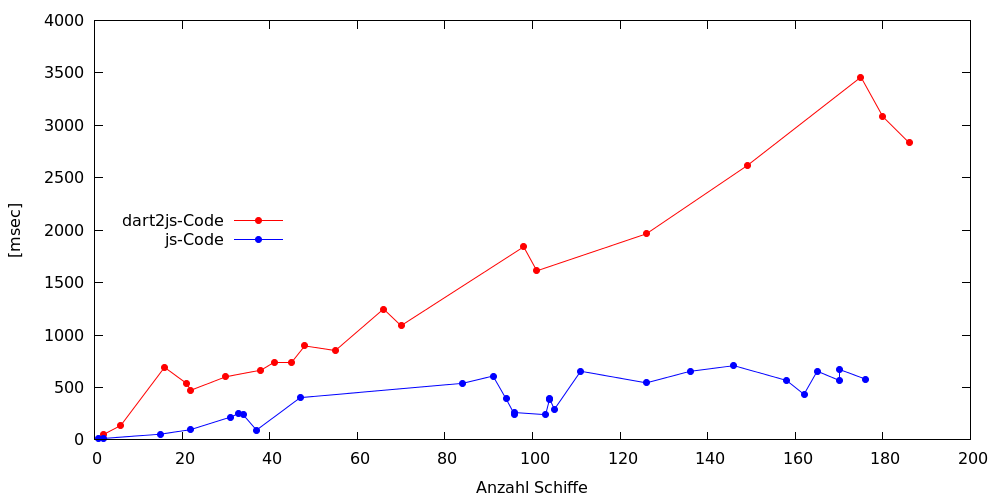
\includegraphics[height=2.3in]{images/Firefox.png}
\end{center}
 \caption{Verarbeitungsdauer in Firefox (HP 530 Notebook PC)}
\end {figure}

%\newpage
In einer zweiten Testserie wurden die Browser-Clients auf einem Apple MacBook Pro 10 mit 2,3 Ghz Intel Core Processor und 8 GB Arbeitsspeicher ausgeführt.
 
\begin {figure}[H]
\begin{center}
  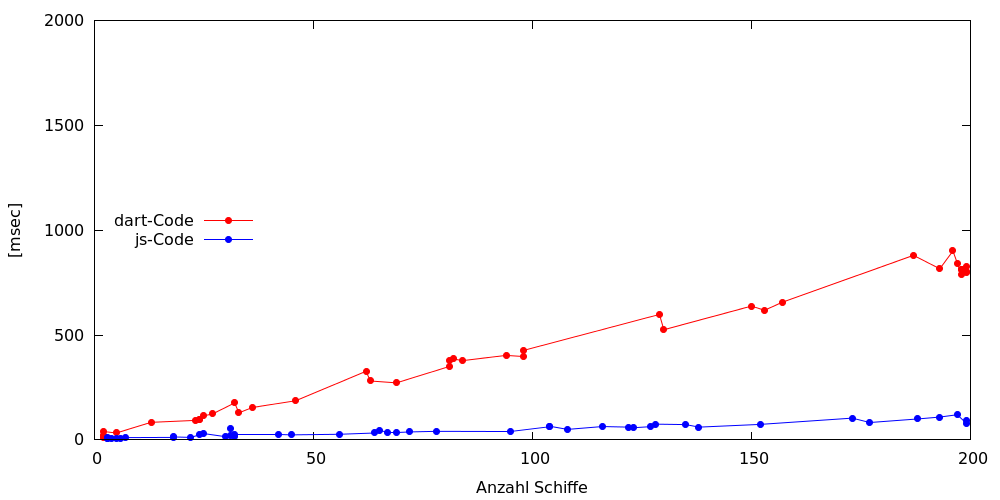
\includegraphics[height=2.3in]{images/DartiumOnMac.png}
\end{center}
 \caption{Verarbeitungsdauer in Dartium (Apple MacBook Pro)}
\end {figure}


\begin {figure}[H]
\begin{center}
  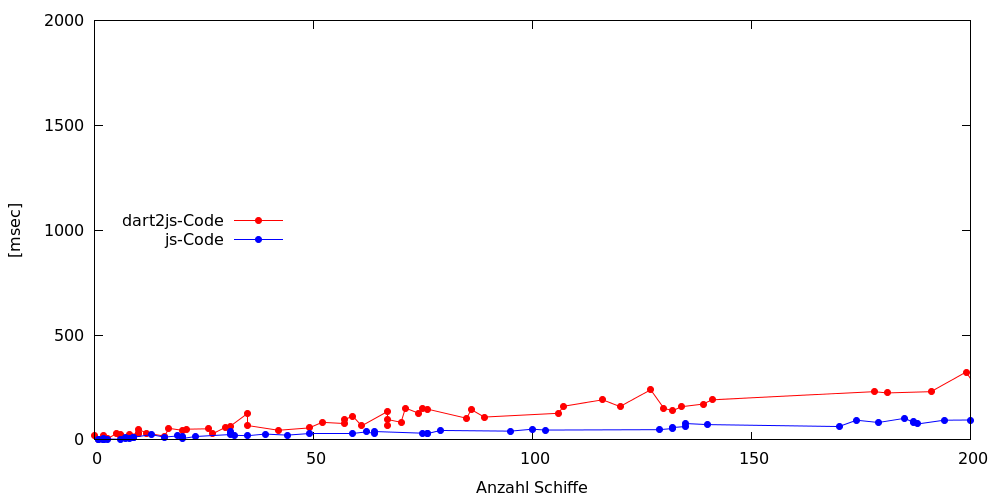
\includegraphics[height=2.3in]{images/ChromeOnMac.png}
\end{center}
 \caption{Verarbeitungsdauer in Chrome (Apple MacBook Pro)}
\end {figure}


\begin {figure}[H]
\begin{center}
  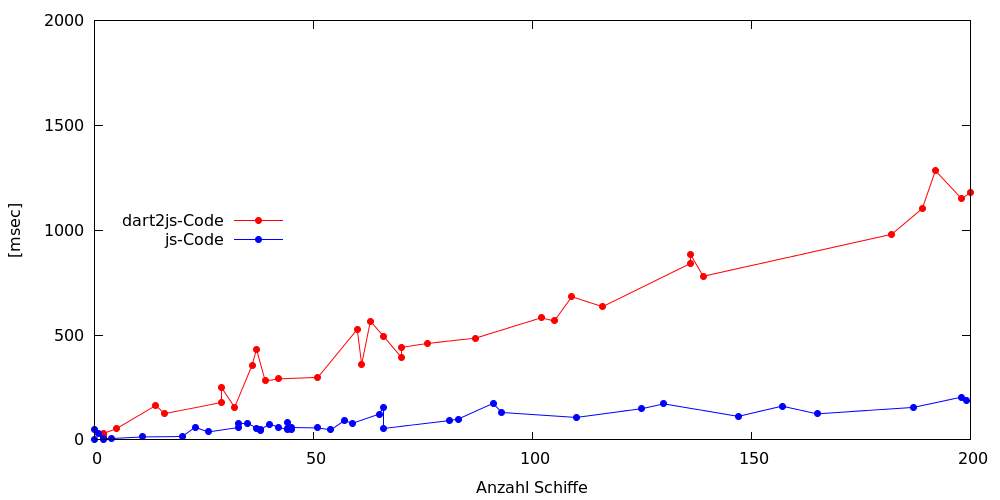
\includegraphics[height=2.3in]{images/FirefoxOnMac.png}
\end{center}
 \caption{Verarbeitungsdauer in Firefox (Apple MacBook Pro)}
\end {figure}

Insgesamt ist erkennbar, dass der Javascript-Code schneller ausgeführt wird als der Dart-Code. Am schnellsten führt die V8-Javascript-Engine in Dartium und Chrome den originären Javascript-Code aus. Firefox mit der Spidermonkey-Javascript-Engine benötigt deutlich länger.\\ Auffällig ist, dass der Dart-Code von der Dart VM in Dartium langsamer ausgeführt wird als der zu Javascript kompilierte Code.
In der zweiten Testserie bestätigen sich diese Ergebnisse. Es ist offensichtlich, dass sich die Geschwindigkeit der Darstellung durch einen leistungsstärkeren Client-Rechner verbessern lässt. Dabei ist deutlich erkennbar, dass der Dart-Client die größte relative Performance-Steigerung erfährt, also am meisten von der zusätzlichen Rechenleistung profitiert.

\subsubsection{Browserunterstützung}
Zusätzlich zu den in den Performance-Tests verwendeten Browsern wurde die Anwendung im InternetExplorer 10 und Safari 6 positiv auf Funktionalität getestet. Das heißt, alle gängigen aktuellen Browser können den zu Javascript kompilierten Dart-Code interpretieren.
%----------------------------------------------------------------------------------------------------------------------------------------------
\chapter{Fazit und Ausblick}\label{Fazit}
%----------------------------------------------------------------------------------------------------------------------------------------------

\section{Die Real-Time-Anwendung}
Der für die Firma Vesseltracker programmierte Prototyp einer Real-Time-Anwendung in Javascript unter Verwendung von node.js mit socket.io ist im Zuge dieser Arbeit Ende Februar 2013 abgeschlossen worden. Die Anwendung soll als zusätzliches Angebot in die Webanwendung der Firma integriert werden. Für einzelne Kunden (z.B. das Maritime Museum Hamburg) ist die Anwendung bereits zugeschnitten und ausgeliefert worden, weitere Kundenprojekte sind geplant.\\

Für die bessere Nutzbarkeit der Anwendung sollte noch eine Möglichkeit geschaffen werden, favorisierte Häfen oder Positionen zu speichern, die per Klick angesteuert werden können, z.B. in einer aufklappbaren Liste.\\
Zur weiteren Optimierung der Anwendung, sollte die Möglichkeit, die Animation der Richtungsdreiecke und Schiffspolygone über css3-Transition-Funktionen zu realisieren, unbedingt weiterverfolgt werden. Damit könnte die vom Browserclient zu erbringende Rechenleistung erheblich reduziert werden, weil die Objekte nicht neu berechnet und erstellt werden müssten, sondern nur über ihre css-Eigenschaften bewegt werden könnten.

%----------------------------------------------------------------------------------------------------------------------------------------------

\section{Vergleich Javascript und Google Dart}
Das Erlernen von Dart ist für Umsteiger von Javascript relativ unkompliziert. Von den vielen Features und Möglichkeiten, die Dart bietet, kommt in der Client-Anwendung nur ein kleiner Teil zum Tragen. Der Fokus lag hier nicht auf den Möglichkeiten von Google Dart, sondern auf der Bewältigung einer konkreten Anforderung. \\
Wie in den Abbildungen zur Struktur der Anwendung erkennbar (Abbildung \ref{fig:Übersicht Dart-Files}), ist mit Dart sehr einfach eine Klassen-Struktur herzustellen. Das macht die Anwendung verständlicher und entsprechend einfacher zu entwerfen, zu schreiben und zu warten.
\\
Hilfreich bei der Entwicklung war der DartEditor als Entwicklungsumgebung. Der Compiler gibt bei Syntax-Fehlern aussagekräftige Fehlermeldungen.\\  
Google Dart befindet sich noch in der Entwicklungsphase, so dass gelegentlich nach den ca. wöchentlichen Versions-Updates von Dart die Anwendung unter der neuen Version nicht mehr lauffähig ist und angepasst werden muss. Belohnt wird dieser Aufwand sozusagen mit einer kontinuierlichen und spürbaren Verbesserung der Performance (Beobachtung im Zeitraum November 2012 bis April 2013).
Das Einbinden existierender Javascript-Bibliotheken mit js-interop erweitert die Nutzungsmöglichen von Dart ganz entscheidend. Das Arbeiten in zwei unterschiedlichen Kontexten (Javascript und Dart) ist am Anfang sehr fehleranfällig. Fehler sind schwierig zu debuggen, weil auch die Debugger (hier Firebug und der Debugger im DartEditor) nur jeweils bis an die Grenzen dieses Kontextes reichen.

Dass in Testserie 2 die Ausführung des Dart-Codes besonders von der besseren Rechenleistung profitiert, lässt vermuten, dass die Kommunikation zwischen den Kontexten innerhalb der Anwendung über Proxies und Callback-Funktionen auch in der Ausführung des Programms einen deutlich höheren Rechenaufwand erzeugt.
Die in dieser Arbeit geschriebene Realtime-Anwendung ist für den ausführenden Client ohnehin sehr rechenintensiv.
\begin{enumerate}
\item werden mit hoher Frequenz Objekte erstellt und gelöscht (besonders durch die Animation der Polygone und Richtungsdreiecke), 
\item werden häufig Events im Dart-Kontext erzeugt (Vessel-Position-Events auf dem Websocket), die Aktionen im Javascript-Kontext notwendig machen und
\item werden bei Benutzeraktionen Events im Javascript-Kontext erzeugt (mouseover-, mouseout- oder moveend-Event), die Aktionen im Dart-Kontext notwendig machen.
\end{enumerate}

Dart bleibt also in der Performance deutlich hinter Javascript zurück. Bei der bisherigen Geschwindigkeit der Entwicklung, insbesondere im Hinblick auf die erlebte Performance-Steigerung, hat Google Dart aber durchaus das Potential, Javascript Konkurrenz zu machen.
Die Einbindung von Javascript-Bibliotheken in Dart ist eine gute Möglichkeit, an die bestehende Web-Welt anzuknüpfen, obwohl der Mehraufwand, der durch die Kommunikation zwischen den beiden Kontexten entsteht sowhl in der Implementierung als auch in der Rechenlast im Browser-Client erheblich ist.\\
Vermutlich wird die Zukunft von Dart sich an zwei Fragen entscheiden:

\begin{itemize}
\item Wie wird die kritische OpenSource Entwicklergemeinde die Sprache aufnehmen, das heißt werden in Zukunft Dart-Bibliotheken in ähnlicher Vielzahl und Diversität entwickelt werden wie in Javascript-Bibliotheken? 
\\
Dr. Axel Rauschmayer beantwortet die Frage, wie quelloffen Google Dart im Vergleich zu Javascript wirklich ist: “
In contrast, Dart is almost proprietary: It is not developed in the open and only shown to the public once it is finished (Brendan Eich calls this ‘delayed-open’). Plus, all of the developers work for Google. It’s great that it is free and eventually open source, both of which will help its popularity. But it probably will never be nearly as open as JavaScript – Google does not have a good track record when it comes to writing specifications for things it open-sources. A recently leaked Android email reminds us that Google is not always as innocent about openness as they sound. Quoting it verbatim:
\begin{itemize}
    \item Do not develop in the open. Instead, make source code available after innovation is complete
    \item Lead device concept: Give early access to the software to partners who build and distribute devices to our specification (ie, Motorola and Verizon). They get a non-contractual time to market advantage and in return they align to our standard.
    \end{itemize}“\cite{google-dart}
\item Wie werden sich die anderen großen Mitspieler auf dem Browsermarkt wie Mozilla, Microsoft und Apple zu Dart positionieren\footnote{http://www.netzwelt.de/news/89916-dart-google-streitet-microsoft-apple-mozilla.html}, das heißt, wird es in Zukunft auch in anderen Browsern Dart Virtual Machines geben?
Dr. Axel Rauschmayer äußert sich dazu: “If you are a competing browser vendor, your prospects for adopting Dart are as follows:
\begin{itemize}
\item    It is difficult to integrate into your existing infrastructure (as you couldn’t give early feedback).
\item    Its development is mainly controlled by Google.
\item    You give Google a head start of over two years.
\end{itemize}
“\cite{google-dart}.
\end{itemize}

%--------------------------------------------------------------------------------------------------------------------------------------------


\bibliographystyle{alphadin_martin}
\bibliography{literatur}


%---------------------------------------------------------------------------------------------------------------------------------------------
\chapter*{Erklärung}

Hiermit versichere ich, dass ich die vorliegende Arbeit selbstständig verfasst und keine anderen als die angegebenen Quellen und Hilfsmittel benutzt habe, dass alle Stellen der Arbeit, die wörtlich oder sinngemäß aus anderen Quellen übernommen wurden, als solche kenntlich gemacht und dass die Arbeit in gleicher oder ähnlicher Form noch keiner Prüfungsbehörde vorgelegt wurde.

\vspace{3cm}
Ort, Datum \hspace{5cm} Unterschrift\\

\end{document}